
% slide-6.tex

\documentclass[dvipdfmx,notheorems,t]{beamer}

\usepackage{docmute}

% settings.tex

\AtBeginSection[]{\frame[t]{\frametitle{目次}
  \tableofcontents[currentsection,hideallsubsections]}}

\AtBeginSubsection[]{\frame[t]{\frametitle{目次}
  \tableofcontents[currentsection,sectionstyle=show/hide,
  currentsubsection,subsectionstyle=show/shaded/hide]}}

\usefonttheme{professionalfonts}
\usetheme{Madrid}

\setbeamercovered{transparent=30} 
% \setbeamertemplate{navigation symbols}{}
\setbeamertemplate{frametitle}[default][left]
\setbeamertemplate{frametitle continuation}{}
\setbeamertemplate{enumerate items}[square]
\setbeamertemplate{caption}[numbered]

\let\oldframe\frame
\renewcommand\frame[1][t,allowdisplaybreaks,allowframebreaks]{\oldframe[#1]}

\addtobeamertemplate{block begin}{\setlength{\abovedisplayskip}{2.5pt}}

\usepackage{bxdpx-beamer}
\usepackage{pxjahyper}
\usepackage{minijs}

\usepackage{amsmath}
\usepackage{amssymb}
\usepackage{amsthm}
\usepackage{bm}
\usepackage{physics}

% Set the path to the figure
\graphicspath{{fig/}}

\usepackage{multirow}

% Add space in the table
\usepackage{cellspace}

% Add space in the table
\setlength\cellspacetoplimit{5pt}
\setlength\cellspacebottomlimit{5pt}

\usepackage{url}

% \hypersetup{
%   colorlinks = true,
%   urlcolor = blue,
%   linkcolor = black,
%   citecolor = green
% }

\DeclareMathOperator*{\argmax}{arg\,max}
\DeclareMathOperator*{\argmin}{arg\,min}
% \DeclareMathOperator{\Tr}{Tr}
% \DeclareMathOperator{\KL}{KL}
\DeclareMathOperator{\diag}{diag}
\DeclareMathOperator{\sgn}{sgn}
\DeclareMathOperator{\adj}{adj}
\DeclareMathOperator{\EOp}{\mathbb{E}}
\DeclareMathOperator{\HOp}{H}
\DeclareMathOperator{\KLOp}{KL}
\DeclareMathOperator{\VarOp}{Var}
\DeclareMathOperator{\CovOp}{Cov}
\newcommand\E[1]{\EOp \left[ #1 \right]}
\newcommand\Entropy[1]{\HOp \left[ #1 \right]}
\newcommand\MutualInfo[1]{I \left( #1 \right)}
\newcommand\KL[2]{\KLOp \left( #1 \parallel #2 \right)}
\newcommand\Var[1]{\VarOp \left[ #1 \right]}
\newcommand\Cov[2]{\CovOp \left( #1, #2 \right)}

\newcommand\BigO[1]{O \left( #1 \right)}
\newcommand\SmallO[1]{o \left( #1 \right)}

\newcommand\Comb[2]{{}_{#1}C_{#2}}

\newcommand{\middlerel}[1]{\mathrel{}\middle#1\mathrel{}}

\usepackage[T1]{fontenc}
\usepackage[utf8]{inputenc}

\setbeamertemplate{theorems}[numbered]
\theoremstyle{definition}
\newtheorem{theorem}{定理}
\newtheorem{definition}{定義}
\newtheorem{proposition}{命題}
\newtheorem{lemma}{補題}
\newtheorem{corollary}{系}
\newtheorem{conjecture}{予想}
\newtheorem*{remark}{Remark}
\renewcommand{\proofname}{}

\renewcommand{\figurename}{図}
\renewcommand{\tablename}{表}

\renewcommand{\kanjifamilydefault}{\gtdefault}



\title{行列輪講: 第6回 確率分布, ガウス積分}
\author{杉浦 圭祐}
\institute[松谷研究室]{慶應義塾大学理工学部情報工学科 松谷研究室}
\date{\today}

% Always use the \displaystyle
\everymath{\displaystyle}

\begin{document}

\linespread{1.1}

\frame{\titlepage}

\section{}

\begin{frame}[t,allowdisplaybreaks,allowframebreaks]{目次}
\tableofcontents
\end{frame}

\section{概要}

\begin{frame}{このスライドの概要}
\begin{itemize}
  \item 確率分布と, ガウス積分について確認する
  \begin{itemize}
    \item 確率密度関数, ベイズの定理, モーメント
    \item エントロピー, KLダイバージェンス, 相互情報量
    \item 不偏推定量, クラメール・ラオ (Cramér--Rao) の下限
    \item 積分の変数変換, 偶関数と奇関数の積分, ガウス積分
  \end{itemize}
  \item 以下の資料を参考に作成しました:
  \begin{itemize}
    \item パターン認識と機械学習 (上巻)
    \item State Estimation For Robotics
  \end{itemize}
\end{itemize}
\end{frame}

\section{確率分布}

\begin{frame}{確率密度関数 (Probability Density Function; PDF)}
\begin{itemize}
  \item 確率変数$x$が, ある\textcolor{red}{確率密度関数}$p(x)$に従うとする.
  \item $p(x)$は, $[a, b]$の範囲で定義されるとする.
  \item $p(x)$は, 2つの条件を満たす:
  \begin{align*}
    p(x) \ge 0, \quad \int_a^b p(x) \dd{x} = 1
  \end{align*}
\end{itemize}
\end{frame}

\begin{frame}{確率密度関数と確率}
\begin{itemize}
  \item 確率密度と確率は別物である.
  \item $x$が, $[c, d]$の範囲をとる\textcolor{red}{確率}を, $\Pr(c \le x \le d)$とする.
  \begin{align*}
    \Pr(c \le x \le d) = \int_c^d p(x) \dd{x}
  \end{align*}
  \item $\Pr(c \le x \le d)$は, 以下の図で, 影がかかった部分である.
\end{itemize}

\begin{figure}
  \centering
  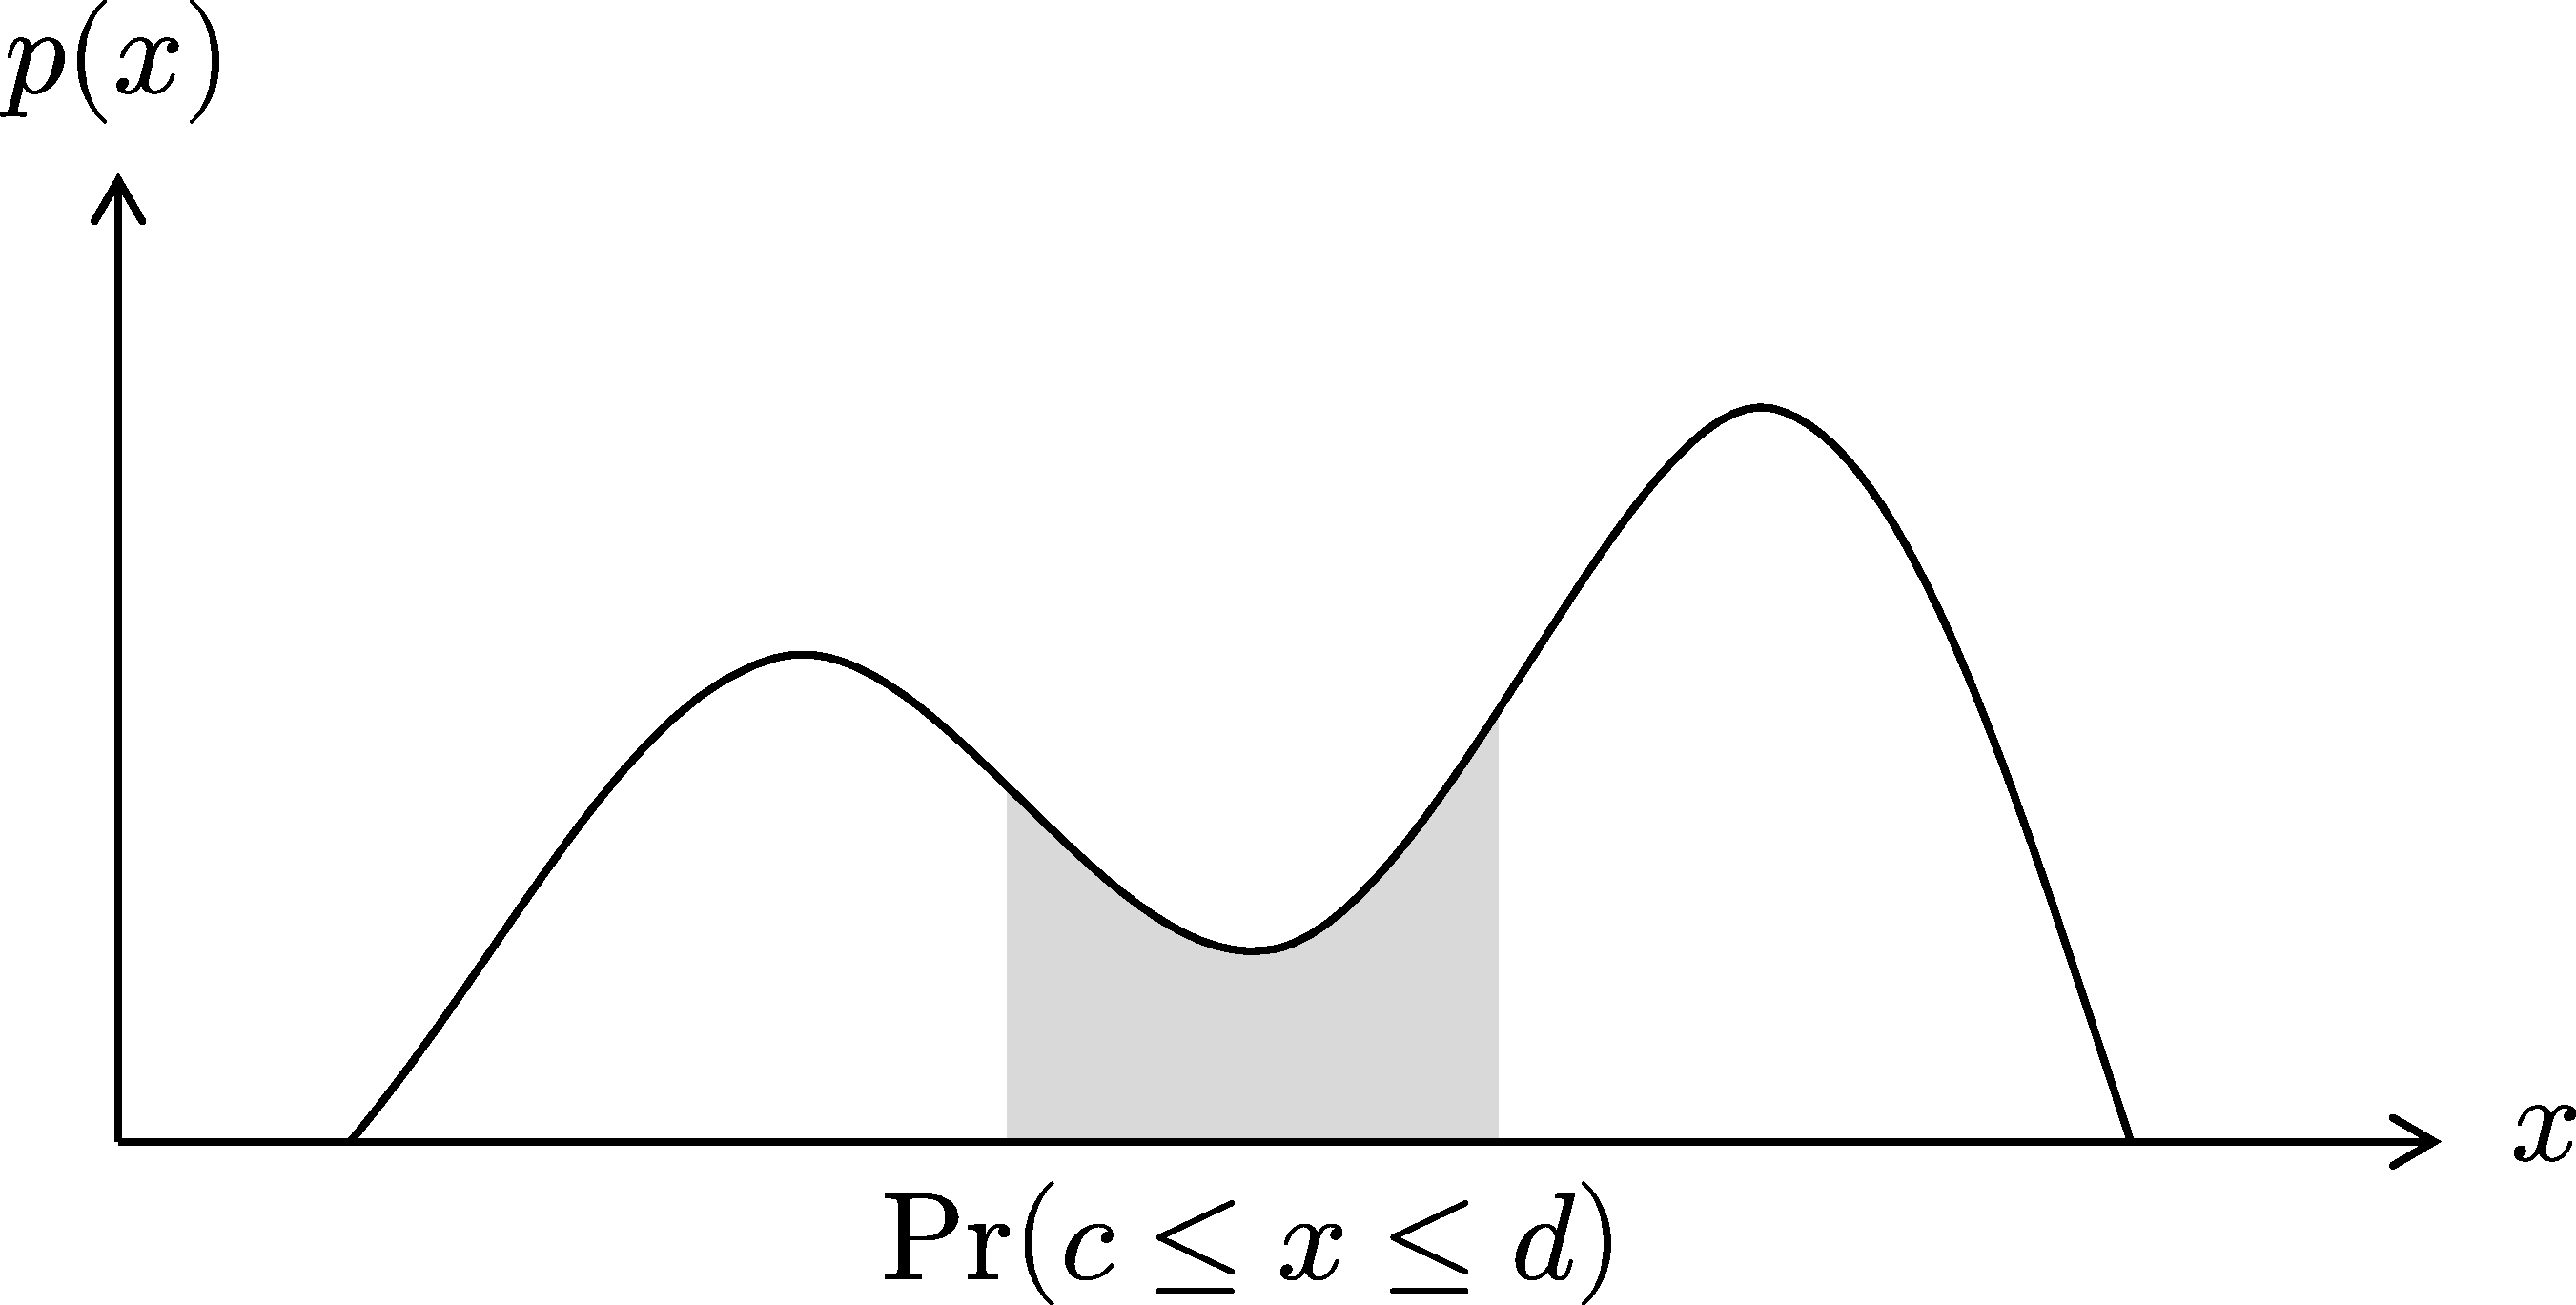
\includegraphics[keepaspectratio, width=0.5\linewidth]{probability-density.pdf}
\end{figure}
\end{frame}

\begin{frame}{条件付き確率分布 (Conditional Probability)}
\begin{itemize}
  \item 確率変数$x \in [a, b]$, $y \in [r, s]$を考える.
  \item $y$に条件付けられた, $x$の確率密度関数$p(x \mid y)$を考える.
  \item $p(x \mid y)$を, \textcolor{red}{条件付き確率密度関数}という.
  \item $p(x \mid y)$も, 2つの条件を満たす:
  \begin{align*}
    p(x \mid y) \ge 0, \quad \int_a^b p(x \mid y) \dd{x} = 1
  \end{align*}
\end{itemize}
\end{frame}

\begin{frame}{同時分布 (Joint Probability)}
\begin{itemize}
  \item 複数の確率変数$x_1, x_2, \ldots, x_N$を考える ($x_i \in [a_i, b_i]$).
  \item これらの確率密度関数$p(x_1, x_2, \ldots, x_N)$を考える.
  \item $p(x_1, x_2, \ldots, x_N)$を, \textcolor{red}{同時確率密度関数}という.
  \item 確率変数をまとめて, $\vb{x} = (x_1, x_2, \ldots, x_N)$とかく.
  \item $p(\vb{x})$も, 2つの条件を満たす:
  \begin{align*}
    p(\vb{x}) &= p(x_1, x_2, \ldots, x_N) \ge 0 \\
    \int_{\vb{a}}^{\vb{b}} p(\vb{x}) \dd{\vb{x}}
      &= \int_{a_N}^{b_N} \cdots \int_{a_1}^{b_1}
        p(x_1, \ldots, x_N) \dd{x_1} \cdots \dd{x_N} = 1
  \end{align*}
  \item 積分の範囲は$\vb{a} = (a_1, a_2, \ldots, a_N)$, $\vb{b} = (b_1, b_2, \ldots, b_N)$である.
  \item 確率変数の範囲については, 以後は明記しない.
\end{itemize}
\end{frame}

\begin{frame}{加法定理 (Sum Rule), 周辺化 (Marginalization), 乗法定理}
\begin{itemize}
  \item 確率変数$\vb{x}, \vb{y}$を考える.
  \item 同時分布$p(\vb{x}, \vb{y})$と, \textcolor{red}{周辺分布}$p(\vb{x})$について, 次が成り立つ.
  \item \textcolor{red}{加法定理}, \textcolor{red}{周辺化}, \textcolor{red}{積分消去}とよばれる.
  \begin{align*}
    p(\vb{x}) &= \int p(\vb{x}, \vb{y}) \dd{\vb{y}}
  \end{align*}
  \item 同時分布$p(\vb{x}, \vb{y})$, 条件付き確率分布$p(\vb{x} \mid \vb{y})$, $p(\vb{y} \mid \vb{x})$,
  周辺分布$p(\vb{x})$, $p(\vb{y})$について, 次が成り立つ.
  \item \textcolor{red}{乗法定理}とよばれる.
  \begin{align*}
    p(\vb{x}, \vb{y}) &= p(\vb{x} \mid \vb{y}) p(\vb{y}) = p(\vb{y} \mid \vb{x}) p(\vb{x})
  \end{align*}
  \item 同時分布は, 周辺分布と, 条件付き確率分布に\textcolor{red}{分解}できる.
\end{itemize}
\end{frame}

\begin{frame}{独立 (Independent)}
\begin{itemize}
  \item 確率変数$\vb{x}, \vb{y}$を考える.
  \item $\vb{x}, \vb{y}$が\textcolor{red}{独立}であるとする.
  \item $\vb{y}$は$\vb{x}$の確率分布に ($\vb{x}$は$\vb{y}$の確率分布に) 影響を与えない.
  \item 条件付き確率分布$p(\vb{x} \mid \vb{y})$は, $p(\vb{x})$に等しい.
  \begin{itemize}
    \item $\vb{y}$が与えられても, $\vb{x}$についての確率分布は変化しない.
  \end{itemize}
  \item 同様に, $p(\vb{y} \mid \vb{x})$は, $p(\vb{y})$に等しい.
  \item 同時分布$p(\vb{x}, \vb{y})$を, 個々の確率分布$p(\vb{x})$, $p(\vb{y})$に分解できる.
  \begin{align*}
    p(\vb{x}, \vb{y}) &= p(\vb{x} \mid \vb{y}) p(\vb{y}) = p(\vb{x}) p(\vb{y}) \quad
      (\because p(\vb{x} \mid \vb{y}) = p(\vb{x})) \\
      &= p(\vb{y} \mid \vb{x}) p(\vb{x}) = p(\vb{x}) p(\vb{y}) \quad
      (\because p(\vb{y} \mid \vb{x}) = p(\vb{y}))
  \end{align*}
  \item $p(\vb{x}, \vb{y}) = p(\vb{x}) p(\vb{y})$であれば, $\vb{x}, \vb{y}$は独立である.
\end{itemize}
\end{frame}

\begin{frame}{ベイズの定理 (Bayes' Theorem)}
\begin{itemize}
  \item 確率の乗法定理から, \textcolor{red}{ベイズの定理}が得られる:
  \begin{align*}
    p(\vb{x}, \vb{y}) &= p(\vb{x} \mid \vb{y}) p(\vb{y}) \quad \longrightarrow \quad
    p(\vb{x} \mid \vb{y}) = \frac{p(\vb{y} \mid \vb{x}) p(\vb{x})}{p(\vb{y})}
  \end{align*}
  \item 分母は周辺化としてかける.
  \begin{align*}
    p(\vb{y}) &= p(\vb{y}) \underbrace{\int p(\vb{x} \mid \vb{y}) \dd{\vb{x}}}_{=1}
      = \int p(\vb{x} \mid \vb{y}) p(\vb{y}) \dd{\vb{x}} \\
      &= \int p(\vb{x}, \vb{y}) \dd{\vb{x}}
      = \int p(\vb{y} \mid \vb{x}) p(\vb{x}) \dd{\vb{x}}
  \end{align*}
  \item ベイズの定理は, 次のようになる.
  \begin{align*}
    p(\vb{x} \mid \vb{y}) = \frac{p(\vb{y} \mid \vb{x}) p(\vb{x})}{p(\vb{y})}
      = \frac{p(\vb{y} \mid \vb{x}) p(\vb{x})}{
        \displaystyle \int p(\vb{y} \mid \vb{x}) p(\vb{x}) \dd{\vb{x}}}
  \end{align*}
\end{itemize}
\end{frame}

\begin{frame}{ベイズの定理 (Bayes' Theorem)}
\begin{block}{ベイズの定理}
  \begin{align*}
    p(\vb{x} \mid \vb{y}) = \frac{p(\vb{y} \mid \vb{x}) p(\vb{x})}{p(\vb{y})}
      = \frac{p(\vb{y} \mid \vb{x}) p(\vb{x})}{
        \displaystyle \int p(\vb{y} \mid \vb{x}) p(\vb{x}) \dd{\vb{x}}}
  \end{align*}
  分母は, $p(\vb{x} \mid \vb{y})$が確率分布になるための正規化 ($\vb{x}$による積分が$1$).
\end{block}
\end{frame}

\begin{frame}{ベイズの定理 (Bayes' Theorem)}
\begin{itemize}
  \item ベイズの定理:
  \begin{align*}
    p(\vb{x} \mid \vb{y}) = \frac{p(\vb{y} \mid \vb{x}) p(\vb{x})}{p(\vb{y})}
      = \frac{p(\vb{y} \mid \vb{x}) p(\vb{x})}{
        \displaystyle \int p(\vb{y} \mid \vb{x}) p(\vb{x}) \dd{\vb{x}}}
  \end{align*}
  \item センサデータ$\vb{y}$を手掛かりに, 変数$\vb{x}$を推定したい.
  \begin{itemize}
    \item 例えば, $\vb{y}$はGPSのデータ, $\vb{x}$はGPSの位置.
  \end{itemize}
\end{itemize}

\begin{enumerate}
  \item $\vb{x}$に関する仮説を, \textcolor{red}{事前分布} (Prior) $p(\vb{x})$として決める.
  \item センサのモデルを, $p(\vb{y} \mid \vb{x})$として決める.
  \begin{itemize}
    \item 変数$\vb{x}$のもとで, どのようなセンサデータ$\vb{y}$が得られるのか?
  \end{itemize}
  \item 新たなセンサデータ$\vb{y}$を得たら, $p(\vb{y} \mid \vb{x}) p(\vb{x})$を計算し, 正規化する.
  \item $\vb{y}$を取り込んだ, $\vb{x}$の\textcolor{red}{事後分布} (Posterior) $p(\vb{x} \mid \vb{y})$が得られる.
\end{enumerate}
\end{frame}

\begin{frame}{ベイズの定理 (Bayes' Theorem)}
\begin{itemize}
  \item 2つの変数$\vb{y}_1$, $\vb{y}_2$から, 変数$\vb{x}$の事後分布$p(\vb{x} \mid \vb{y}_1, \vb{y}_2)$を推定したい.
  \begin{align*}
    p(\vb{x} \mid \vb{y}_1, \vb{y}_2) &= \frac{
      p(\vb{y}_1, \vb{y}_2 \mid \vb{x}) p(\vb{x})}{p(\vb{y}_1, \vb{y}_2)}
      \quad (\because \text{ベイズの定理})
  \end{align*}
  \item $\vb{x}$のもとで$\vb{y}_1, \vb{y}_2$が互いに独立なら, 以下が成り立つ:
  \begin{align*}
    p(\vb{y}_1, \vb{y}_2 \mid \vb{x}) &= p(\vb{y}_1 \mid \vb{x}) p(\vb{y}_2 \mid \vb{x})
      = \frac{p(\vb{x} \mid \vb{y}_1) p(\vb{y}_1)}{p(\vb{x})}
      \frac{p(\vb{x} \mid \vb{y}_2) p(\vb{y}_2)}{p(\vb{x})}
  \end{align*}
  \item 上記を代入すれば, 次が得られる.
  \begin{align*}
    p(\vb{x} \mid \vb{y}_1, \vb{y}_2)
      &= \eta \ p(\vb{x} \mid \vb{y}_1) p(\vb{x} \mid \vb{y}_2)
  \end{align*}
  \item $\eta = \frac{p(\vb{y}_1) p(\vb{y}_2)}{p(\vb{y}_1, \vb{y}_2) p(\vb{x})}$は正規化項である.
\end{itemize}
\end{frame}

\begin{frame}{モーメント, 平均, 分散, 歪度, 尖度}
\begin{itemize}
  \item 確率分布$p(x)$の形状ではなく, モーメントだけを扱うことは多々ある.
  \item $\E{f(x)}$を, 関数$f(x)$の, 確率分布$p(x)$のもとでの\textcolor{red}{期待値}とする.
  \begin{align*}
    \E{f(x)} &= \int f(x) p(x) \dd{x}
  \end{align*}
  \item 1次モーメント: \textcolor{red}{平均} $\mu = \E{x}$ (Mean)
  \item 2次モーメント: \textcolor{red}{分散} $\sigma^2 = \Var{x} = \E{(x - \mu)^2}$ (Variance)
  \item 3次モーメント: $\E{(x - \mu)^3}$
  \item 4次モーメント: $\E{(x - \mu)^4}$
  \begin{align*}
    \mu &= \E{x} = \int x p(x) \dd{x} \\
    \sigma^2 &= \Var{x} = \E{(x - \mu)^2} = \int (x - \mu)^2 p(x) \dd{x}
  \end{align*}
\end{itemize}
\end{frame}

\begin{frame}{モーメント, 平均, 分散, 歪度, 尖度}
\begin{itemize}
  \item 確率分布$p(x)$の\textcolor{red}{歪度} (Skewness; わいど):
  \begin{align*}
    \E{\left( \frac{x - \mu}{\sigma} \right)^3} = \frac{\E{\left( x - \mu \right)^3}}{\sigma^3}
      = \frac{\E{\left( x - \mu \right)^3}}{\E{\left( x - \mu \right)^2}^\frac{3}{2}}
  \end{align*}
  \item 確率分布$p(x)$の\textcolor{red}{尖度} (Kurtosis; せんど):
  \begin{align*}
    \E{\left( \frac{x - \mu}{\sigma} \right)^4} = \frac{\E{\left( x - \mu \right)^4}}{\sigma^4}
      = \frac{\E{\left( x - \mu \right)^4}}{\E{\left( x - \mu \right)^2}^2}
  \end{align*}
  \item 尖度は, $\E{\left( \frac{x - \mu}{\sigma} \right)^4} - 3$とすることもある.
  \begin{itemize}
    \item ガウス分布の尖度を$0$とするため.
  \end{itemize}
\end{itemize}
\end{frame}

\begin{frame}{モーメント, 平均, 共分散 (多変数の場合)}
\begin{itemize}
  \item 行列関数$\vb{F}(\vb{x})$の, 確率分布$p(\vb{x})$のもとでの期待値:
  \begin{align*}
    \E{\vb{F}(\vb{x})} &= \int \vb{F}(\vb{x}) p(\vb{x}) \dd{\vb{x}}
  \end{align*}
  \item $\E{\vb{F}(\vb{x})}$の$(i, j)$成分は, $\vb{F}$の$(i, j)$成分$f_{ij}$を用いて,
  \begin{align*}
    \left( \E{\vb{F}(\vb{x})} \right)_{ij} &= \E{f_{ij}(\vb{x})}
      = \int f_{ij}(\vb{x}) p(\vb{x}) \dd{\vb{x}}
  \end{align*}
  \item 平均$\vb*{\mu}$と\textcolor{red}{共分散}$\vb{\Sigma}$ (Covariance) は, 次のようにかける.
  \begin{align*}
    \vb*{\mu} &= \E{\vb{x}} = \int \vb{x} p(\vb{x}) \dd{\vb{x}} \\
    \vb{\Sigma} &= \Var{\vb{x}} = \E{\left( \vb{x} - \vb*{\mu} \right) \left( \vb{x} - \vb*{\mu} \right)^\top}
      = \int \left( \vb{x} - \vb*{\mu} \right) \left( \vb{x} - \vb*{\mu} \right)^\top p(\vb{x}) \dd{\vb{x}}
  \end{align*}
\end{itemize}
\end{frame}

\begin{frame}{モーメント, 平均, 共分散 (多変数の場合)}
\begin{itemize}
  \item 2つの変数$\vb{x}, \vb{y}$について, 次が成り立つ.
  \begin{align*}
    \E{\vb{x} + \vb{y}} = \E{\vb{x}} + \E{\vb{y}}
  \end{align*}
  \item $n$個の変数$\vb{x}_1, \ldots, \vb{x}_n$について, 次が成り立つ.
  \begin{align*}
    \E{\sum_{i = 1}^n \vb{x}_i} = \sum_{i = 1}^n \E{\vb{x}_i}
  \end{align*}
  \item 和の期待値と, 期待値の和が等しい.
  \item スカラの場合にも, 同様に成立する.
  \begin{align*}
    \E{x + y} &= \E{x} + \E{y}, \quad
    \E{\sum_{i = 1}^n x_i} = \sum_{i = 1}^n \E{x_i}
  \end{align*}
\end{itemize}
\end{frame}

\begin{frame}{モーメント, 平均, 共分散 (多変数の場合)}
\begin{itemize}
  \item 変数$\vb{x}$と, ある定数$\vb{A}$について, 次が成り立つ.
  \begin{align*}
    \E{\vb{A} \vb{x}} = \vb{A} \E{\vb{x}}, \quad
    \E{\vb{x} \vb{A}} = \E{\vb{x}} \vb{A}
  \end{align*}
  \item 変数$\vb{x}$と, ある定数$\vb{a}$について, 次が成り立つ.
  \begin{align*}
    \E{\vb{x} + \vb{a}} = \E{\vb{x}} + \vb{a}
  \end{align*}
  \item スカラの場合にも, 同様に成立する.
  \begin{align*}
    \E{a x} = a \E{x}, \quad
    \E{x + a} = \E{x} + a
  \end{align*}
\end{itemize}
\end{frame}

\begin{frame}{モーメント, 平均, 共分散 (多変数の場合)}
\begin{itemize}
  \item 確率分布$p(\vb{x})$の共分散が$\vb{\Sigma} = \Var{\vb{x}}$であるとする.
  \item $\vb{y} = \vb{A} \vb{x}$としたとき, $p(\vb{y})$の共分散$\Var{\vb{y}}$は,
  \begin{align*}
    \Var{\vb{y}}
    &= \E{\left( \vb{y} - \E{\vb{y}} \right) \left( \vb{y} - \E{\vb{y}} \right)^\top} \\
    &= \text{\color{red} (練習問題)} \\
    % &= \E{\left( \vb{A} \vb{x} - \E{\vb{A} \vb{x}} \right)
    %   \left( \vb{A} \vb{x} - \E{\vb{A} \vb{x}} \right)^\top} \\
    % &= \E{\vb{A} \left( \vb{x} - \E{\vb{x}} \right) \left( \vb{x} - \E{\vb{x}} \right)^\top \vb{A}^\top} \\
    % &= \vb{A} \E{\left( \vb{x} - \E{\vb{x}} \right) \left( \vb{x} - \E{\vb{x}} \right)^\top} \vb{A}^\top
    &= \vb{A} \vb{\Sigma} \vb{A}^\top
  \end{align*}
  \item ただし, $\E{\vb{A} \vb{x}} = \vb{A} \E{\vb{x}}$.
  \item 同様に, $p(x)$の分散が$\sigma^2$であれば, $y = ax$の分散は$a^2 \sigma^2$.
\end{itemize}
\end{frame}

\begin{frame}{モーメント, 平均, 共分散 (多変数の場合)}
\begin{itemize}
  \item 確率分布$p(\vb{x})$の共分散が$\vb{\Sigma} = \Var{\vb{x}}$であるとする.
  \item $\vb{y} = \vb{x} + \vb{a}$としたとき ($\vb{a}$は定数), $p(\vb{y})$の共分散$\Var{\vb{y}}$は,
  \begin{align*}
    \Var{\vb{y}}
    &= \E{\left( \vb{y} - \E{\vb{y}} \right) \left( \vb{y} - \E{\vb{y}} \right)^\top} \\
    &= \E{\left( \vb{x} + \vb{a} - \E{\vb{x} + \vb{a}} \right)
      \left( \vb{x} + \vb{a} - \E{\vb{x} + \vb{a}} \right)^\top} \\
    &= \E{\left( \vb{x} + \vb{a} - \E{\vb{x}} - \vb{a} \right)
      \left( \vb{x} + \vb{a} - \E{\vb{x}} - \vb{a} \right)^\top} \\
    &= \E{\left( \vb{x} - \E{\vb{x}} \right) \left( \vb{x} - \E{\vb{x}} \right)^\top} = \vb{\Sigma}
  \end{align*}
  \item ただし, $\E{\vb{x} + \vb{a}} = \E{\vb{x}} + \vb{a}$.
  \item 同様に, $p(x)$の分散が$\sigma^2$であれば, $y = x + a$の分散も$\sigma^2$.
\end{itemize}
\end{frame}

\begin{frame}{モーメント, 平均, 共分散 (多変数の場合)}
\begin{itemize}
  \item 確率分布$p(\vb{x})$の共分散$\vb{\Sigma} = \Var{\vb{x}}$について, 次が成り立つ.
  \begin{align*}
    \vb{\Sigma} &= \Var{\vb{x}} = \E{\vb{x} \vb{x}^\top} - \E{\vb{x}} \E{\vb{x}}^\top
      = \E{\vb{x} \vb{x}^\top} - \vb*{\mu} \vb*{\mu}^\top
  \end{align*}
  \item スカラの場合は, 次のようになる.
  \begin{align*}
    \sigma^2 &= \Var{x} = \E{x^2} - \left( \E{x} \right)^2 = \E{x^2} - \mu^2
  \end{align*}
  \item \textcolor{red}{練習問題.}
  % \item 以下のように示せる.
  % \begin{align*}
  %   \vb{\Sigma} &= \E{\left( \vb{x} - \vb*{\mu} \right) \left( \vb{x} - \vb*{\mu} \right)^\top} \\
  %     &= \E{\vb{x} \vb{x}^\top} - \E{\vb{x} \vb*{\mu}^\top}
  %       - \E{\vb*{\mu} \vb{x}^\top} + \E{\vb*{\mu} \vb*{\mu}^\top} \\
  %     &= \E{\vb{x} \vb{x}^\top} - \E{\vb{x}} \vb*{\mu}^\top
  %       - \vb*{\mu} \E{\vb{x}}^\top + \vb*{\mu} \vb*{\mu}^\top \\
  %     &= \E{\vb{x} \vb{x}^\top} - \vb*{\mu} \vb*{\mu}^\top
  %       - \vb*{\mu} \vb*{\mu}^\top + \vb*{\mu} \vb*{\mu}^\top
  % \end{align*}
\end{itemize}
\end{frame}

\begin{frame}{独立 (Independent), 無相関 (Uncorrelated)}
\begin{itemize}
  \item 以下が成り立つとき, $\vb{x}, \vb{y}$は\textcolor{red}{独立}である:
  \begin{align*}
    p(\vb{x}, \vb{y}) &= p(\vb{x}) p(\vb{y})
  \end{align*}
  \item 以下が成り立つとき, $\vb{x}, \vb{y}$は\textcolor{red}{無相関}である:
  \begin{align*}
    \E{\vb{x} \vb{y}^\top} &= \E{\vb{x}} \E{\vb{y}}^\top
  \end{align*}
  \item 独立$\Rightarrow$無相関は成り立つが, 無相関$\Rightarrow$独立は\textcolor{red}{成り立たない}.
  \item 独立$\Rightarrow$無相関は, \textcolor{red}{練習問題.}
  % \begin{align*}
  %   \E{\vb{x} \vb{y}^\top} &= \iint \vb{x} \vb{y}^\top p(\vb{x}, \vb{y}) \dd{\vb{x}} \dd{\vb{y}}
  %     = \iint \vb{x} \vb{y}^\top p(\vb{x}) p(\vb{y}) \dd{\vb{x}} \dd{\vb{y}} \, (\because \text{独立}) \\
  %     &= \int \vb{x} p(\vb{x}) \dd{\vb{x}} \int \vb{y}^\top p(\vb{y}) \dd{\vb{y}}
  %     = \E{\vb{x}} \E{\vb{y}}^\top
  % \end{align*}
\end{itemize}
\end{frame}

\begin{frame}{相互共分散 (Cross-covariance)}
\begin{itemize}
  \item $\vb{x}$と$\vb{y}$との間の\textcolor{red}{相互共分散}$\Cov{\vb{x}}{\vb{y}}$は, 次のようにかける.
  \begin{align*}
    \Cov{\vb{x}}{\vb{y}}
      = \E{\left( \vb{x} - \E{\vb{x}} \right) \left( \vb{y} - \E{\vb{y}} \right)^\top}
      &= \E{\vb{x} \vb{y}^\top} - \E{\vb{x}} \E{\vb{y}}^\top
  \end{align*}
  \item 左辺を展開すれば, 次のように示せる.
  \begin{align*}
    & \E{\left( \vb{x} - \E{\vb{x}} \right) \left( \vb{y} - \E{\vb{y}} \right)^\top} \\
      &= \E{\vb{x} \vb{y}^\top} - \E{\vb{x} \E{\vb{y}}^\top}
        - \E{\E{\vb{x}} \vb{y}^\top} + \E{\E{\vb{x}} \E{\vb{y}}^\top} \\
      &= \E{\vb{x} \vb{y}^\top} - \E{\vb{x}} \E{\vb{y}}^\top
        - \E{\vb{x}} \E{\vb{y}}^\top + \E{\vb{x}} \E{\vb{y}}^\top
  \end{align*}
  \item $\vb{x}, \vb{y}$が無相関 ($\E{\vb{x} \vb{y}^\top} = \E{\vb{x}} \E{\vb{y}}^\top$) であれば, 相互共分散は$\vb{0}$.
  \item 独立$\Rightarrow$無相関であるから, 独立であれば, 相互共分散は$\vb{0}$.
\end{itemize}
\end{frame}

\begin{frame}{相互共分散 (Cross-covariance)}
\begin{itemize}
  \item $\Cov{\vb{x}}{\vb{y}} = \Cov{\vb{y}}{\vb{x}}^\top$が成り立つ:
  \begin{align*}
    \Cov{\vb{x}}{\vb{y}}
      &= \E{\left( \vb{x} - \E{\vb{x}} \right) \left( \vb{y} - \E{\vb{y}} \right)^\top} \\
      &= \E{\left( \vb{y} - \E{\vb{y}} \right) \left( \vb{x} - \E{\vb{x}} \right)^\top}^\top
      = \Cov{\vb{y}}{\vb{x}}^\top
  \end{align*}
  \item $\Cov{\vb{x} + \vb{y}}{\vb{z}} = \Cov{\vb{x}}{\vb{z}} + \Cov{\vb{y}}{\vb{z}}$も成り立つ:
  {\small \begin{align*}
    \Cov{\vb{x} + \vb{y}}{\vb{z}}
      &= \E{\left( \vb{x} + \vb{y} - \E{\vb{x} + \vb{y}} \right)
        \left( \vb{z} - \E{\vb{z}} \right)^\top} \\
      &= \E{\left( \left( \vb{x} - \E{\vb{x}} \right) + \left( \vb{y} - \E{\vb{y}} \right) \right)
        \left( \vb{z} - \E{\vb{z}} \right)^\top} \\
      &= \E{\left( \vb{x} - \E{\vb{x}} \right) \left( \vb{z} - \E{\vb{z}} \right)^\top}
        + \E{\left( \vb{y} - \E{\vb{y}} \right) \left( \vb{z} - \E{\vb{z}} \right)^\top} \\
      &= \Cov{\vb{x}}{\vb{z}} + \Cov{\vb{y}}{\vb{z}}
  \end{align*}}
  \item ただし, $\E{\vb{x} + \vb{y}} = \E{\vb{x}} + \E{\vb{y}}$.
\end{itemize}
\end{frame}

\begin{frame}{相互共分散 (Cross-covariance)}
\begin{itemize}
  \item $\Cov{\vb{A} \vb{x}}{\vb{B} \vb{y}} = \vb{A} \Cov{\vb{x}}{\vb{y}} \vb{B}^\top$も成り立つ:
  {\small \begin{align*}
    \Cov{\vb{A} \vb{x}}{\vb{B} \vb{y}}
    &= \E{\left( \vb{A} \vb{x} - \E{\vb{A} \vb{x}} \right)
      \left( \vb{B} \vb{y} - \E{\vb{B} \vb{y}} \right)^\top} \\
    &= \E{\vb{A} \left( \vb{x} - \E{\vb{x}} \right)
      \left( \vb{B} \left( \vb{y} - \E{\vb{y}} \right) \right)^\top} \\
    &= \E{\vb{A} \left( \vb{x} - \E{\vb{x}} \right)
      \left( \vb{y} - \E{\vb{y}} \right)^\top \vb{B}^\top} \\
    &= \vb{A} \E{\left( \vb{x} - \E{\vb{x}} \right)
      \left( \vb{y} - \E{\vb{y}} \right)^\top} \vb{B}^\top
    = \vb{A} \Cov{\vb{x}}{\vb{y}} \vb{B}^\top
  \end{align*}}
  \item $\Cov{\vb{x} + \vb{a}}{\vb{y} + \vb{b}} = \Cov{\vb{x}}{\vb{y}}$も成り立つ:
  \begin{align*}
    \Cov{\vb{x} + \vb{a}}{\vb{y} + \vb{b}}
    &= \E{\left( \vb{x} + \vb{a} - \E{\vb{x} + \vb{a}} \right)
      \left( \vb{y} + \vb{b} - \E{\vb{y} + \vb{b}} \right)} \\
    &= \E{\left( \vb{x} + \vb{a} - \E{\vb{x}} - \vb{a} \right)
      \left( \vb{y} + \vb{b} - \E{\vb{y}} - \vb{b} \right)} \\
    &= \E{\left( \vb{x} - \E{\vb{x}} \right)
      \left( \vb{y} - \E{\vb{y}} \right)^\top} = \Cov{\vb{x}}{\vb{y}}
  \end{align*}
\end{itemize}
\end{frame}

\begin{frame}{共分散と相互共分散}
\begin{itemize}
  \item $\vb{x}, \vb{y}$の共分散を$\Var{\vb{x}}, \Var{\vb{y}}$, 相互共分散を$\Cov{\vb{x}}{\vb{y}}$とする.
  \item $\vb{z} = \vb{x} + \vb{y}$としたとき, $p(\vb{z})$の共分散$\Var{\vb{z}}$は,
  {\small \begin{align*}
    & \E{\left( \vb{z} - \E{\vb{z}} \right) \left( \vb{z} - \E{\vb{z}} \right)^\top} \\
    &= \E{\left( \vb{x} + \vb{y} - \E{\vb{x} + \vb{y}} \right)
      \left( \vb{x} + \vb{y} - \E{\vb{x} + \vb{y}} \right)^\top} \\
    &= \E{\left( \left( \vb{x} - \E{\vb{x}} \right) + \left( \vb{y} - \E{\vb{y}} \right) \right)
      \left( \left( \vb{x} - \E{\vb{x}} \right) + \left( \vb{y} - \E{\vb{y}} \right) \right)^\top} \\
    &= \E{\left( \vb{x} - \E{\vb{x}} \right) \left( \vb{x} - \E{\vb{x}} \right)^\top}
      + \E{\left( \vb{y} - \E{\vb{y}} \right) \left( \vb{y} - \E{\vb{y}} \right)^\top} \\
    & \quad + \E{\left( \vb{x} - \E{\vb{x}} \right) \left( \vb{y} - \E{\vb{y}} \right)^\top}
      + \E{\left( \vb{y} - \E{\vb{y}} \right) \left( \vb{x} - \E{\vb{x}} \right)^\top} \\
    &= \Var{\vb{x}} + \Var{\vb{y}} + \Cov{\vb{x}}{\vb{y}} + \Cov{\vb{y}}{\vb{x}}
  \end{align*}}
  \item 同様に, $z = x + y$の分散は, $\Var{z} = \Var{x} + \Var{y} + 2 \Cov{x}{y}$.
\end{itemize}
\end{frame}

\begin{frame}{平均, 共分散, 相互共分散 (1変数の場合)}
\begin{block}{平均, 共分散, 相互共分散 (1変数の場合)}
  \begin{align*}
    \E{x + y} &= \E{x} + \E{y} \\
    \E{x + a} &= \E{x} + a \\
    \E{ax} &= a \E{x} \\
    \Var{x} &= \E{(x - \E{x})^2} \\
    \Var{ax} &= a^2 \Var{x} \\
    \Var{x + a} &= \Var{x} \\
    \Var{x} &= \E{x^2} - \E{x}^2
  \end{align*}
\end{block}
\end{frame}

\begin{frame}{平均, 共分散, 相互共分散 (1変数の場合)}
\begin{block}{平均, 共分散, 相互共分散 (1変数の場合)}
  \begin{align*}
    \Cov{x}{y} &= \E{(x - \E{x}) (y - \E{y})} \\
    \Cov{x}{y} &= \E{xy} - \E{x} \E{y} \\
    \Cov{x + y}{z} &= \Cov{x}{z} + \Cov{y}{z} \\
    \Cov{ax}{by} &= ab \Cov{x}{y} \\
    \Cov{x + a}{y + b} &= \Cov{x}{y} \\
    \Var{x + y} &= \Var{x} + \Var{y} + 2 \Cov{x}{y}
  \end{align*}
\end{block}
\end{frame}

\begin{frame}{平均, 共分散, 相互共分散 (1変数の場合)}
\begin{block}{無相関 (Uncorrelated)}
  $x, y$が無相関であれば, $\E{xy} = \E{x} \E{y}$. \\
  独立であれば ($p(x, y) = p(x) p(y)$), 無相関.
  \begin{align*}
    \Cov{x}{y} &= 0 \\
    \Var{x + y} &= \Var{x} + \Var{y}
  \end{align*}
\end{block}
\end{frame}

\begin{frame}{平均, 共分散, 相互共分散 (多変数の場合)}
\begin{block}{平均, 共分散, 相互共分散 (多変数の場合)}
  \begin{align*}
    \E{\vb{x} + \vb{y}} &= \E{\vb{x}} + \E{\vb{y}} \\
    \E{\vb{x} + \vb{a}} &= \E{\vb{x}} + \vb{a} \\
    \E{\vb{A} \vb{x}} &= \vb{A} \E{\vb{x}} \\
    \E{\vb{x} \vb{A}} &= \E{\vb{x}} \vb{A} \\
    \Var{\vb{x}} &= \E{\left( \vb{x} - \E{\vb{x}} \right) \left( \vb{x} - \E{\vb{x}} \right)^\top} \\
    \Var{\vb{A} \vb{x}} &= \vb{A} \Var{\vb{x}} \vb{A}^\top \\
    \Var{\vb{x} + \vb{a}} &= \Var{\vb{x}} \\
    \Var{\vb{x}} &= \E{\vb{x} \vb{x}^\top} - \E{\vb{x}} \E{\vb{x}}^\top
  \end{align*}
\end{block}
\end{frame}

\begin{frame}{平均, 共分散, 相互共分散 (多変数の場合)}
\begin{block}{平均, 共分散, 相互共分散 (多変数の場合)}
  \begin{align*}
    \Cov{\vb{x}}{\vb{y}} &= \E{\left( \vb{x} - \E{\vb{x}} \right) \left( \vb{y} - \E{\vb{y}} \right)^\top} \\
    \Cov{\vb{x}}{\vb{y}} &= \E{\vb{x} \vb{y}^\top} - \E{\vb{x}} \E{\vb{y}}^\top \\
    \Cov{\vb{x}}{\vb{y}} &= \Cov{\vb{y}}{\vb{x}}^\top \\
    \Cov{\vb{x} + \vb{y}}{\vb{z}} &= \Cov{\vb{x}}{\vb{z}} + \Cov{\vb{y}}{\vb{z}} \\
    \Cov{\vb{A} \vb{x}}{\vb{B} \vb{y}} &= \vb{A} \Cov{\vb{x}}{\vb{y}} \vb{B}^\top \\
    \Cov{\vb{x} + \vb{a}}{\vb{y} + \vb{b}} &= \Cov{\vb{x}}{\vb{y}} \\
    \Var{\vb{x} + \vb{y}} &= \Var{\vb{x}} + \Var{\vb{y}}
      + \Cov{\vb{x}}{\vb{y}} + \Cov{\vb{y}}{\vb{x}}
  \end{align*}
\end{block}
\end{frame}

\begin{frame}{平均, 共分散, 相互共分散 (多変数の場合)}
\begin{block}{無相関 (Uncorrelated)}
  $\vb{x}, \vb{y}$が無相関であれば, $\E{\vb{x} \vb{y}^\top} = \E{\vb{x}} \E{\vb{y}}^\top$. \\
  独立であれば ($p(\vb{x}, \vb{y}) = p(\vb{x}) p(\vb{y})$), 無相関.
  \begin{align*}
    \Cov{\vb{x}}{\vb{y}} &= \vb{0} \\
    \Var{\vb{x} + \vb{y}} &= \Var{\vb{x}} + \Var{\vb{y}}
  \end{align*}
\end{block}
\end{frame}

\begin{frame}{平均, 共分散, 相互共分散の関係 (発展)}
\begin{block}{二次形式}
  {\small \begin{align*}
    \E{\left( \vb{A} \vb{x} + \vb{b} \right)^\top \left( \vb{C} \vb{x} + \vb{d} \right)}
      = \tr(\vb{A} \Var{\vb{x}} \vb{C}^\top)
      + \left( \vb{A} \E{\vb{x}} + \vb{b} \right)^\top
        \left( \vb{C} \E{\vb{x}} + \vb{d} \right)
  \end{align*}}
\end{block}

\begin{itemize}
  \item これまでにみてきた公式を駆使すれば, 導出できる.
  \item 上式を基に, 次が直ちに得られる:
  \begin{align*}
    \E{\vb{x}^\top \vb{x}} &= \tr(\Var{\vb{x}}) + \E{\vb{x}}^\top \E{\vb{x}} \\
    \E{\vb{x}^\top \vb{C} \vb{x}} &= \tr(\vb{C} \Var{\vb{x}}) + \E{\vb{x}}^\top \vb{C} \E{\vb{x}} \\
    \E{\left( \vb{A} \vb{x} \right)^\top \left( \vb{A} \vb{x} \right)}
      &= \tr(\vb{A} \Var{\vb{x}} \vb{A}^\top)
      + \left( \vb{A} \E{\vb{x}} \right)^\top \left( \vb{A} \E{\vb{x}} \right) \\
    \E{\left( \vb{x} + \vb{a} \right)^\top \left( \vb{x} + \vb{a} \right)}
      &= \tr(\Var{\vb{x}}) + \left( \E{\vb{x}} + \vb{a} \right)^\top \left( \E{\vb{x}} + \vb{a} \right)
  \end{align*}
\end{itemize}
\end{frame}

\begin{frame}{平均, 共分散, 相互共分散の関係 (発展)}
\begin{itemize}
  \item $\E{\cdot}$の中身がスカラーであることを考えて, 式を変形すると,
  {\small \begin{align*}
    & \E{\left( \vb{A} \vb{x} + \vb{b} \right)^\top \left( \vb{C} \vb{x} + \vb{d} \right)} \\
    &= \E{\tr(\left( \vb{C} \vb{x} + \vb{d} \right) \left( \vb{A} \vb{x} + \vb{b} \right)^\top)}
    = \tr(\E{\left( \vb{C} \vb{x} + \vb{d} \right) \left( \vb{A} \vb{x} + \vb{b} \right)^\top}) \\
    &= \tr(\Cov{\vb{C} \vb{x} + \vb{d}}{\vb{A} \vb{x} + \vb{b}}
      + \E{\vb{C} \vb{x} + \vb{d}} \E{\vb{A} \vb{x} + \vb{b}}^\top) \\
    &= \tr(\Cov{\vb{C} \vb{x} + \vb{d}}{\vb{A} \vb{x} + \vb{b}})
      + \tr(\E{\vb{C} \vb{x} + \vb{d}} \E{\vb{A} \vb{x} + \vb{b}}^\top) \\
    &= \tr(\Cov{\vb{C} \vb{x} + \vb{d}}{\vb{A} \vb{x} + \vb{b}})
      + \E{\vb{A} \vb{x} + \vb{b}}^\top \E{\vb{C} \vb{x} + \vb{d}} \\
    &= \tr(\Cov{\vb{C} \vb{x} + \vb{d}}{\vb{A} \vb{x} + \vb{b}})
      + \left( \vb{A} \E{\vb{x}} + \vb{b} \right)^\top
      \left( \vb{C} \E{\vb{x}} + \vb{d} \right)
  \end{align*}}
  \item ただし, 以下の関係を用いた:
  {\small \begin{align*}
    \E{\tr(\vb{A})} = \tr(\E{\vb{A}}), \quad
    \tr(\vb{a} \vb{b}^\top) = \vb{b}^\top \vb{a} \\
    \E{\vb{x} \vb{y}^\top} = \Cov{\vb{x}}{\vb{y}} + \E{\vb{x}} \E{\vb{y}}^\top
  \end{align*}}
\end{itemize}
\end{frame}

\begin{frame}{平均, 共分散, 相互共分散の関係 (発展)}
\begin{itemize}
  \item 続いて, $\tr(\Cov{\vb{C} \vb{x} + \vb{d}}{\vb{A} \vb{x} + \vb{b}})
    = \tr(\vb{A} \Var{\vb{x}} \vb{C}^\top)$を示す.
  \begin{align*}
    \tr(\Cov{\vb{C} \vb{x} + \vb{d}}{\vb{A} \vb{x} + \vb{b}})
    &= \tr(\Cov{\vb{C} \vb{x}}{\vb{A} \vb{x}}) \\
    &= \tr(\vb{C} \Cov{\vb{x}}{\vb{x}} \vb{A}^\top) \\
    &= \tr(\vb{C} \Var{\vb{x}} \vb{A}^\top)
    = \tr(\vb{A} \Var{\vb{x}} \vb{C}^\top)
  \end{align*}
  \item ただし, 以下の関係を用いた:
  \begin{gather*}
    \Cov{\vb{x} + \vb{a}}{\vb{y} + \vb{b}} = \Cov{\vb{x}}{\vb{y}} \\
    \Cov{\vb{A} \vb{x}}{\vb{B} \vb{y}} = \vb{A} \Cov{\vb{x}}{\vb{y}} \vb{B}^\top \\
    \Cov{\vb{x}}{\vb{x}} = \E{\left( \vb{x} - \E{\vb{x}} \right)
      \left( \vb{x} - \E{\vb{x}} \right)^\top} = \Var{\vb{x}} \\
    \tr(\vb{A}^\top) = \tr(\vb{A}), \quad \Var{\vb{x}}^\top = \Var{\vb{x}}
  \end{gather*}
\end{itemize}
\end{frame}

\begin{frame}{平均, 共分散, 相互共分散の関係 (発展)}
\begin{block}{二次関数}
  \begin{align*}
    \E{\left( \vb{A} \vb{x} + \vb{b} \right) \left( \vb{C} \vb{x} + \vb{d} \right)^\top}
    = \vb{A} \Var{\vb{x}} \vb{C}^\top
    + \left( \vb{A} \E{\vb{x}} + \vb{b} \right)
      \left( \vb{C} \E{\vb{x}} + \vb{d} \right)^\top
  \end{align*}
\end{block}

\begin{itemize}
  \item 上式を基に, 次が直ちに得られる:
  \begin{align*}
    \E{\vb{x} \vb{x}^\top} &= \Var{\vb{x}} + \E{\vb{x}} \E{\vb{x}}^\top \\
    \E{\left( \vb{A} \vb{x} \right) \left( \vb{A} \vb{x} \right)^\top}
      &= \vb{A} \left( \Var{\vb{x}} + \E{\vb{x}} \E{\vb{x}}^\top \right) \vb{A}^\top \\
    \E{\left( \vb{x} + \vb{a} \right) \left( \vb{x} + \vb{a} \right)^\top}
      &= \Var{\vb{x}} + \left( \E{\vb{x}} + \vb{a} \right) \left( \E{\vb{x}} + \vb{a} \right)^\top
  \end{align*}
\end{itemize}
\end{frame}

\begin{frame}{平均, 共分散, 相互共分散の関係 (発展)}
\begin{itemize}
  \item 次のように変形できる:
  \begin{align*}
    & \E{\left( \vb{A} \vb{x} + \vb{b} \right) \left( \vb{C} \vb{x} + \vb{d} \right)^\top} \\
    &= \text{\color{red} (練習問題)} \\
    % &= \Cov{\vb{A} \vb{x} + \vb{b}}{\vb{C} \vb{x} + \vb{d}}
    %   + \E{\vb{A} \vb{x} + \vb{b}} \E{\vb{C} \vb{x} + \vb{d}}^\top \\
    % &= \Cov{\vb{A} \vb{x}}{\vb{C} \vb{x}}
    %   + \left( \vb{A} \E{\vb{x}} + \vb{b} \right) \left( \vb{C} \E{\vb{x}} + \vb{d} \right)^\top \\
    % &= \vb{A} \Cov{\vb{x}}{\vb{x}} \vb{C}^\top
    %   + \left( \vb{A} \E{\vb{x}} + \vb{b} \right) \left( \vb{C} \E{\vb{x}} + \vb{d} \right)^\top \\
    &= \vb{A} \Var{\vb{x}} \vb{C}^\top
      + \left( \vb{A} \E{\vb{x}} + \vb{b} \right) \left( \vb{C} \E{\vb{x}} + \vb{d} \right)^\top
  \end{align*}
  \item ただし, 以下の関係を用いた:
  {\small \begin{gather*}
    \E{\vb{x} \vb{y}^\top} = \Cov{\vb{x}}{\vb{y}} + \E{\vb{x}} \E{\vb{y}}^\top \\
    \Cov{\vb{x} + \vb{a}}{\vb{y} + \vb{b}} = \Cov{\vb{x}}{\vb{y}}, \quad
    \Cov{\vb{A} \vb{x}}{\vb{B} \vb{y}} = \vb{A} \Cov{\vb{x}}{\vb{y}} \vb{B}^\top \\
    \Cov{\vb{x}}{\vb{x}} = \E{\left( \vb{x} - \E{\vb{x}} \right)
      \left( \vb{x} - \E{\vb{x}} \right)^\top} = \Var{\vb{x}}
  \end{gather*}}
\end{itemize}
\end{frame}

\begin{frame}{平均, 共分散, 相互共分散の関係 (発展)}
\begin{block}{二次関数}
  \begin{align*}
    \E{\vb{x} \vb{a}^\top \vb{x}} &= \left( \Var{\vb{x}} + \E{\vb{x}} \E{\vb{x}}^\top \right) \vb{a} \\
    \E{\vb{x}^\top \vb{a} \vb{x}^\top} &= \vb{a}^\top \left( \Var{\vb{x}} + \E{\vb{x}} \E{\vb{x}}^\top \right)
  \end{align*}
\end{block}

\begin{itemize}
  \item 次のように確認できる:
  \begin{align*}
    \E{\vb{x} \left( \vb{a}^\top \vb{x} \right)} &= \E{\vb{x} \vb{x}^\top \vb{a}}
      = \E{\vb{x} \vb{x}^\top} \vb{a} \\
      &= \left( \Var{\vb{x}} + \E{\vb{x}} \E{\vb{x}}^\top \right) \vb{a} \\
    \E{\left( \vb{x}^\top \vb{a} \right) \vb{x}^\top} &= \E{\vb{a}^\top \vb{x} \vb{x}^\top}
      = \vb{a}^\top \E{\vb{x} \vb{x}^\top} \\
      &= \vb{a}^\top \left( \Var{\vb{x}} + \E{\vb{x}} \E{\vb{x}}^\top \right)
  \end{align*}
\end{itemize}
\end{frame}

\begin{frame}{イェンセンの不等式 (Jensen's Inequality)}
\begin{itemize}
  \item \textcolor{red}{下に凸な}関数$f(\vb{x})$を考える.
  \item $p(\vb{x})$を, $\int p(\vb{x}) \dd{\vb{x}} = 1$をみたす関数とする.
  \item $f(\vb{x}), p(\vb{x})$について, \textcolor{red}{イェンセンの不等式}が成り立つ:
  \begin{align*}
    \int f(\vb{x}) p(\vb{x}) \dd{\vb{x}} &\ge f \left( \int \vb{x} p(\vb{x}) \dd{\vb{x}} \right)
  \end{align*}
  \item $p(\vb{x})$を確率分布とすれば, 期待値$\E{\cdot}$を用いて, 次のようにかける:
  \begin{align*}
    \E{f(\vb{x})} &\ge f(\E{\vb{x}})
  \end{align*}
  \item $f(\vb{x})$が\textcolor{red}{上に凸}であれば, 次が成り立つ (不等号が逆になる):
  \begin{align*}
    \int f(\vb{x}) p(\vb{x}) \dd{\vb{x}} &\le f \left( \int \vb{x} p(\vb{x}) \dd{\vb{x}} \right) \\
    \E{f(\vb{x})} &\le f(\E{\vb{x}})
  \end{align*}
\end{itemize}
\end{frame}

\begin{frame}{イェンセンの不等式 (Jensen's Inequality)}
\begin{itemize}
  \item \textcolor{red}{下に凸}であれば, 任意の2点を結ぶ直線が, 上側にある (\textcolor{red}{凸関数}, 左).
  \begin{itemize}
    \item $x^2$, $x \ln x$, $\frac{1}{x} \ (x > 0)$, $\tan x \ (0 < x < \frac{\pi}{2})$など
  \end{itemize}
  \item \textcolor{red}{上に凸}であれば, 任意の2点を結ぶ直線が, 下側にある (\textcolor{red}{凹関数}, 右).
  \begin{itemize}
    \item $\ln x$, $\tan x \ (-\frac{\pi}{2} < x < 0)$など
  \end{itemize}
\end{itemize}

\begin{figure}
  \centering
  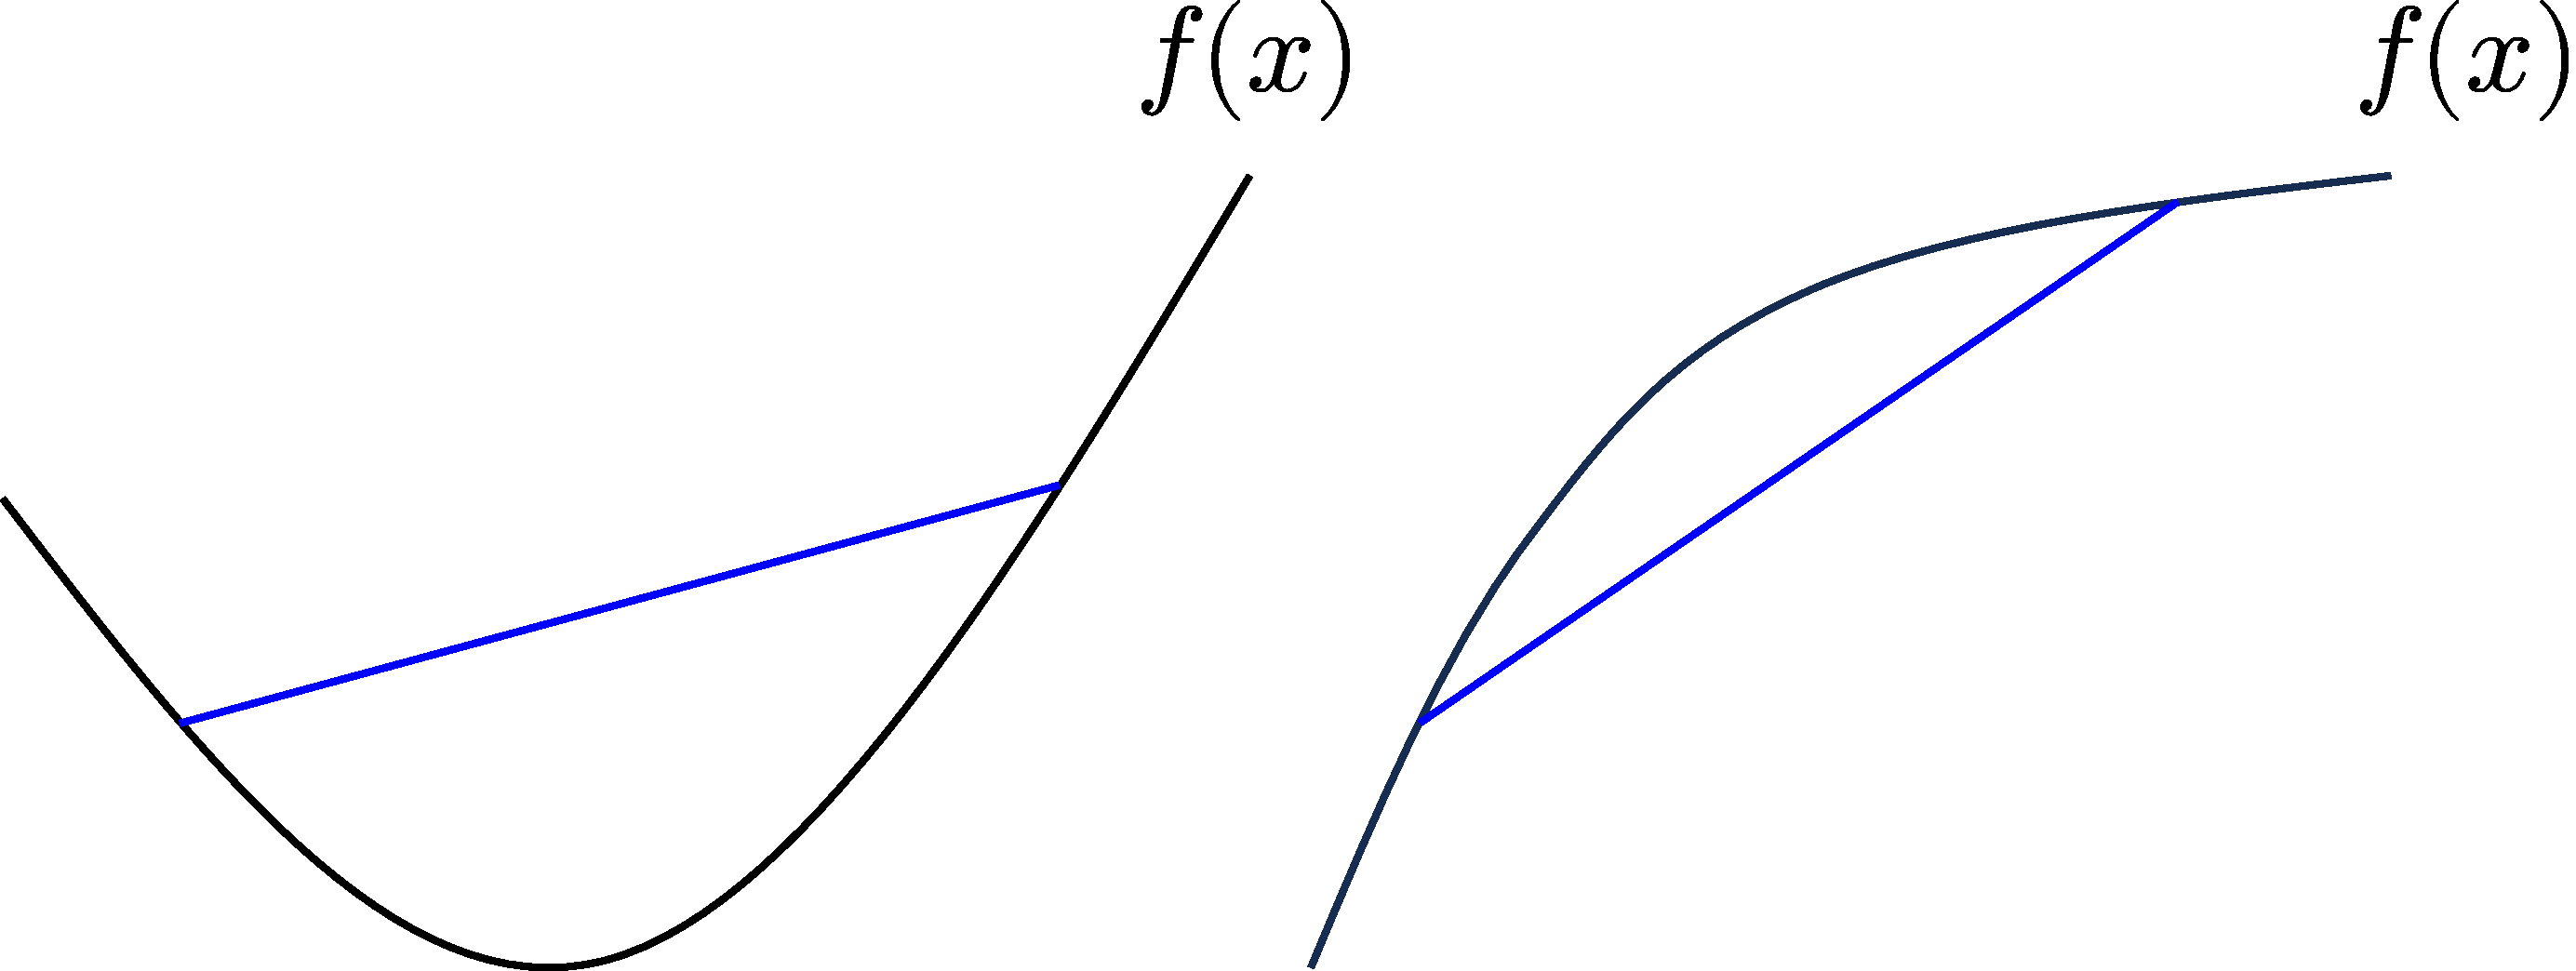
\includegraphics[keepaspectratio, width=0.75\linewidth]{convex-function.pdf}
\end{figure}
\end{frame}

\begin{frame}{エントロピー (Entropy)}
\begin{itemize}
  \item 確率分布$p(\vb{x})$について, 次の量$\Entropy{\vb{x}}$を考える.
  \begin{align*}
    \Entropy{\vb{x}} &= -\E{\ln p(\vb{x})} = - \int p(\vb{x}) \ln p(\vb{x}) \dd{\vb{x}}
  \end{align*}
  \item $\Entropy{\vb{x}}$を, \textcolor{red}{エントロピー}, \textcolor{red}{シャノン情報量}, \textcolor{red}{平均情報量}とよぶ.
  \item 直感的には, $\vb{x}$を, どのくらい予測しづらいのかを表す.
  \begin{itemize}
    \item $\vb{x}$が離散変数であれば, 一様分布のときにエントロピーが最大である.
    \item $\vb{x}$が連続変数であれば, 正規分布 (ガウス分布) のときに最大.
    \item この証明には, 変分計算が必要である.
  \end{itemize}
\end{itemize}
\end{frame}

\begin{frame}{条件付きエントロピー (Conditional Entropy)}
\begin{itemize}
  \item 同時分布$p(\vb{x}, \vb{y})$のエントロピー$\Entropy{\vb{x}, \vb{y}}$を考える.
  \begin{align*}
    \Entropy{\vb{x}, \vb{y}} &= -\E{\ln p(\vb{x}, \vb{y})}
      = - \iint p(\vb{x}, \vb{y}) \ln p(\vb{x}, \vb{y}) \dd{\vb{x}} \dd{\vb{y}}
  \end{align*}
  \item $p(\vb{x}, \vb{y}) = p(\vb{y} \mid \vb{x}) p(\vb{x})$のように分解できるので, 代入すれば
  \begin{align*}
    \Entropy{\vb{x}, \vb{y}}
      &= - \iint p(\vb{y} \mid \vb{x}) p(\vb{x})
        \left( \ln p(\vb{y} \mid \vb{x}) + \ln p(\vb{x}) \right) \dd{\vb{x}} \dd{\vb{y}} \\
      &= - \iint p(\vb{x}, \vb{y}) \ln p(\vb{y} \mid \vb{x}) \dd{\vb{x}} \dd{\vb{y}} \\
      & \quad - \int p(\vb{x}) \ln p(\vb{x}) \dd{\vb{x}}
        \underbrace{\int p(\vb{y} \mid \vb{x}) \dd{\vb{y}}}_{=1} \\
      &= \Entropy{\vb{y} \mid \vb{x}} + \Entropy{\vb{x}}
  \end{align*}
\end{itemize}
\end{frame}

\begin{frame}{条件付きエントロピー (Conditional Entropy)}
\begin{itemize}
  \item 条件付き確率分布$p(\vb{y} \mid \vb{x})$について, $\Entropy{\vb{y} \mid \vb{x}}$を次のように定める.
  \begin{align*}
    \Entropy{\vb{y} \mid \vb{x}} &= -\E{\ln p(\vb{y} \mid \vb{x})}
      = - \iint p(\vb{x}, \vb{y}) \ln p(\vb{y} \mid \vb{x}) \dd{\vb{x}} \dd{\vb{y}}
  \end{align*}
  \item $\Entropy{\vb{y} \mid \vb{x}}$を, \textcolor{red}{条件付きエントロピー}とよぶ.
  \item 次が成り立つ:
  \begin{align*}
    \Entropy{\vb{x}, \vb{y}} &= \Entropy{\vb{y} \mid \vb{x}} + \Entropy{\vb{x}}
      = \Entropy{\vb{x} \mid \vb{y}} + \Entropy{\vb{y}}
  \end{align*}
  \item $\Entropy{\vb{x}}$: $\vb{x}$の予測しづらさ
  \item $\Entropy{\vb{x}, \vb{y}}$: $\vb{x}$と$\vb{y}$の予測しづらさ
  \item $\Entropy{\vb{y} \mid \vb{x}}$: $\vb{x}$が既知であるときの, $\vb{y}$の予測しづらさ
\end{itemize}
\end{frame}

\begin{frame}{カルバック--ライブラーダイバージェンス (Kullback-Leibler Divergence)}
\begin{itemize}
  \item 2つの確率分布$p(\vb{x}), q(\vb{x})$があるとき, 次の量$\KL{p}{q}$を考える.
  \begin{align*}
    \KL{p}{q} &= -\E{\ln \frac{q(\vb{x})}{p(\vb{x})}}
      = -\int p(\vb{x}) \ln \frac{q(\vb{x})}{p(\vb{x})} \dd{\vb{x}}
  \end{align*}
  \item $\KL{p}{q}$を, \textcolor{red}{カルバック--ライブラーダイバージェンス}とよぶ.
  \item 長いので, \textcolor{red}{KLダイバージェンス}ともよぶ.
  \item 確率分布$p(\vb{x})$と$q(\vb{x})$との距離のような概念である.
  \item $\KL{p}{q} \neq \KL{q}{p}$であるから, 厳密な距離ではない.
\end{itemize}
\end{frame}

\begin{frame}{カルバック--ライブラーダイバージェンス (Kullback-Leibler Divergence)}
\begin{itemize}
  \item カルバック--ライブラーダイバージェンス:
  \begin{align*}
    \KL{p}{q} &= -\E{\ln \frac{q(\vb{x})}{p(\vb{x})}}
      = -\int p(\vb{x}) \ln \frac{q(\vb{x})}{p(\vb{x})} \dd{\vb{x}}
  \end{align*}
  % \item $-\ln x$は下に凸だから, イェンセンの不等式より ($\E{f(x)} \le f(\E{x})$)
  % \begin{align*}
  %   \KL{p}{q} &= -\E{\ln \frac{q(\vb{x})}{p(\vb{x})}}
  %     \ge -\ln \E{\frac{q(\vb{x})}{p(\vb{x})}} \\
  %     &= -\ln \int p(\vb{x}) \frac{q(\vb{x})}{p(\vb{x})} \dd{\vb{x}}
  %     = -\ln \int q(\vb{x}) \dd{\vb{x}} = -\ln 1 = 0
  % \end{align*}
  \item $\KL{p}{q} \ge 0$ (\textcolor{red}{練習問題}).
  \item $\forall \vb{x} \ p(\vb{x}) = q(\vb{x})$のときのみ$0$.
\end{itemize}
\end{frame}

\begin{frame}{相互情報量 (Mutual Information)}
\begin{itemize}
  \item 確率変数$\vb{x}, \vb{y}$について, 次の量$\MutualInfo{\vb{x}, \vb{y}}$を考える.
  \begin{align*}
    \MutualInfo{\vb{x}, \vb{y}} &= \E{\ln \frac{p(\vb{x}, \vb{y})}{p(\vb{x}) p(\vb{y})}}
      = \iint p(\vb{x}, \vb{y}) \ln \frac{p(\vb{x}, \vb{y})}{p(\vb{x}) p(\vb{y})} \dd{\vb{x}} \dd{\vb{y}}
  \end{align*}
  \item $\MutualInfo{\vb{x}, \vb{y}}$を, \textcolor{red}{相互情報量}とよぶ.
  \item $\vb{x}$ ($\vb{y}$) を得たとき, $\vb{y}$ ($\vb{x}$) についての情報がどのくらい増えるか.
  \item $\vb{x}, \vb{y}$が独立であれば ($p(\vb{x}, \vb{y}) = p(\vb{x}) p(\vb{y})$), $\MutualInfo{\vb{x}, \vb{y}} = 0$.
  \begin{align*}
    \MutualInfo{\vb{x}, \vb{y}}
      &= \iint p(\vb{x}, \vb{y}) \ln \frac{p(\vb{x}) p(\vb{y})}{p(\vb{x}) p(\vb{y})} \dd{\vb{x}} \dd{\vb{y}}
      = \iint p(\vb{x}, \vb{y}) \ln 1 \dd{\vb{x}} \dd{\vb{y}} = 0
  \end{align*}
  \item $\vb{x}, \vb{y}$が独立であれば, $\vb{x}$ ($\vb{y}$) のことが分かっても,
  $\vb{y}$ ($\vb{x}$) については何の情報ももたらさない.
\end{itemize}
\end{frame}

\begin{frame}{相互情報量 (Mutual Information)}
\begin{itemize}
  \item 相互情報量$\MutualInfo{\vb{x}, \vb{y}}$:
  \begin{align*}
    \MutualInfo{\vb{x}, \vb{y}} &= \E{\ln \frac{p(\vb{x}, \vb{y})}{p(\vb{x}) p(\vb{y})}}
      = \iint p(\vb{x}, \vb{y}) \ln \frac{p(\vb{x}, \vb{y})}{p(\vb{x}) p(\vb{y})} \dd{\vb{x}} \dd{\vb{y}}
  \end{align*}
  \item エントロピー$\Entropy{\vb{x}}, \Entropy{\vb{y}}, \Entropy{\vb{x}, \vb{y}}$を使って, 次のようにかける.
  \begin{align*}
    \MutualInfo{\vb{x}, \vb{y}} &= \Entropy{\vb{x}} + \Entropy{\vb{y}} - \Entropy{\vb{x}, \vb{y}}
  \end{align*}
  \item $\Entropy{\vb{x}, \vb{y}} = \Entropy{\vb{y} \mid \vb{x}} + \Entropy{\vb{x}}
  = \Entropy{\vb{x} \mid \vb{y}} + \Entropy{\vb{y}}$であるから,
  \begin{align*}
    \MutualInfo{\vb{x}, \vb{y}} &= \Entropy{\vb{y}} - \Entropy{\vb{y} \mid \vb{x}}
      = \Entropy{\vb{x}} - \Entropy{\vb{x} \mid \vb{y}}
  \end{align*}
  \item $\Entropy{\vb{y}}$: $\vb{y}$の予測しづらさ
  \item $\Entropy{\vb{y} \mid \vb{x}}$: $\vb{x}$が既知であるときの, $\vb{y}$の予測しづらさ
  \item $\MutualInfo{\vb{x}, \vb{y}}$: $\vb{x}$が分かったとき, $\vb{y}$がどのくらい予測しやすくなるか
\end{itemize}
\end{frame}

\begin{frame}{相互情報量 (Mutual Information)}
\begin{itemize}
  \item 相互情報量$\MutualInfo{\vb{x}, \vb{y}}$:
  \begin{align*}
    \MutualInfo{\vb{x}, \vb{y}} &= \E{\ln \frac{p(\vb{x}, \vb{y})}{p(\vb{x}) p(\vb{y})}}
      = \iint p(\vb{x}, \vb{y}) \ln \frac{p(\vb{x}, \vb{y})}{p(\vb{x}) p(\vb{y})} \dd{\vb{x}} \dd{\vb{y}}
  \end{align*}
  \item カルバック--ライブラーダイバージェンスを用いると,
  \begin{align*}
    \MutualInfo{\vb{x}, \vb{y}} &= -\E{\ln \frac{p(\vb{x}) p(\vb{y})}{p(\vb{x}, \vb{y})}}
      = \KL{p(\vb{x}, \vb{y})}{p(\vb{x}) p(\vb{y})}
  \end{align*}
  \item KLダイバージェンスの性質 ($\ge 0$) から, $\MutualInfo{\vb{x}, \vb{y}} \ge 0$.
  \item $\forall \vb{x}, \vb{y} \ p(\vb{x}, \vb{y}) = p(\vb{x}) p(\vb{y})$のとき (独立であるとき) に限って$0$.
  \item 確率変数$\vb{x}, \vb{y}$が, 独立に近いかどうかを表している.
\end{itemize}
\end{frame}

\begin{frame}{不偏推定量 (Unbiased Estimate)}
\begin{itemize}
  \item パラメータ$\vb*{\theta}$をもつ$\vb{x}$の確率分布$p(\vb{x} \mid \vb*{\theta})$を考える.
  \item この確率分布から, 観測データが得られたとする.
  \begin{align*}
    \vb{x}_\mathrm{meas} \gets p(\vb{x} \mid \vb*{\theta})
  \end{align*}
  \item 観測データ$\vb{x}_\mathrm{meas}$を基に, パラメータ$\vb*{\theta}$を推定したい.
  \item パラメータ$\vb*{\theta}$の推定量$\hat{\vb*{\theta}}$が,
  \textcolor{red}{不偏推定量}であるとき, 以下が成り立つ:
  \begin{align*}
    \E{\hat{\vb*{\theta}}} = \vb*{\theta}
      \quad \longrightarrow \quad \E{\hat{\vb*{\theta}} - \vb*{\theta}} = \vb{0}
  \end{align*}
  \item 推定量の期待値$\E{\hat{\vb*{\theta}}}$が, 真のパラメータ$\vb*{\theta}$に一致する (偏りがない).
\end{itemize}
\end{frame}

\begin{frame}{不偏推定量 (Unbiased Estimate)}
\begin{itemize}
  \item 例えば, 平均$\vb*{\mu}$と共分散$\vb{\Sigma}$をもつ$\vb{x}$の確率分布
  $p(\vb{x} \mid \vb*{\mu}, \vb{\Sigma})$から, $N$個の観測データが得られたとする:
  \begin{gather*}
    \left\{ \vb{x}_{1, \mathrm{meas}}, \ldots, \vb{x}_{N, \mathrm{meas}} \right\}
      \gets p(\vb{x} \mid \vb*{\mu}, \vb{\Sigma}) \\
    \E{\vb{x}_\mathrm{meas}} = \vb*{\mu}, \quad
    \E{\left( \vb{x}_\mathrm{meas} - \vb*{\mu} \right)
      \left( \vb{x}_\mathrm{meas} - \vb*{\mu} \right)^\top} = \vb{\Sigma}
  \end{gather*}
  \item 観測データは, \textcolor{red}{互いに独立}であるとする.
  \item 観測データ$\{ \vb{x}_{i, \mathrm{meas}} \}$を基に,
  分布の平均$\vb*{\mu}$と共分散$\vb{\Sigma}$を推定したい.
\end{itemize}
\end{frame}

\begin{frame}{不偏推定量 (Unbiased Estimate)}
\begin{itemize}
  \item 平均$\vb*{\mu}$と共分散$\vb{\Sigma}$をもつ$\vb{x}$の確率分布
  $p(\vb{x} \mid \vb*{\mu}, \vb{\Sigma})$から, $N$個の観測データが得られたとする:
  \begin{align*}
    \left\{ \vb{x}_{1, \mathrm{meas}}, \ldots, \vb{x}_{N, \mathrm{meas}} \right\}
      \gets p(\vb{x} \mid \vb*{\mu}, \vb{\Sigma})
  \end{align*}
  \item 観測データ$\{ \vb{x}_{i, \mathrm{meas}} \}$を基に,
  分布の平均$\vb*{\mu}$と共分散$\vb{\Sigma}$を推定したい.
  \item 平均と共分散の\textcolor{red}{不偏推定量}は, 次のようになる:
  \begin{align*}
    \hat{\vb*{\mu}} &= \frac{1}{N} \sum_{i = 1}^N \vb{x}_{i, \mathrm{meas}}, \quad
    \hat{\vb{\Sigma}} = \frac{1}{N - 1} \sum_{i = 1}^N
      \left( \vb{x}_{i, \mathrm{meas}} - \hat{\vb*{\mu}} \right)
      \left( \vb{x}_{i, \mathrm{meas}} - \hat{\vb*{\mu}} \right)^\top
  \end{align*}
  \item 共分散については, 分母が$N$の代わりに\textcolor{red}{$N - 1$となる}ことに注意.
  \item $\hat{\vb*{\mu}}$は, \textcolor{red}{標本平均}という.
  \item $\hat{\vb{\Sigma}}$は, \textcolor{red}{不偏分散}という (分母が$N$のときは, \textcolor{red}{標本分散}).
\end{itemize}
\end{frame}

\begin{frame}{不偏推定量 (Unbiased Estimate)}
\begin{itemize}
  \item 不偏分散は, 分母が$N$の代わりに$N - 1$になる (少し大きく補正):
  \begin{align*}
    \hat{\vb{\Sigma}} = \frac{1}{N - 1} \sum_{i = 1}^N
      \left( \vb{x}_{i, \mathrm{meas}} - \hat{\vb*{\mu}} \right)
      \left( \vb{x}_{i, \mathrm{meas}} - \hat{\vb*{\mu}} \right)^\top
  \end{align*}
  \item 共分散の計算に, 真の平均$\vb*{\mu}$ではなく,
  \textcolor{red}{観測データから計算された}標本平均$\hat{\vb*{\mu}}$を使っているから.
  \begin{itemize}
    \item 観測データ$\vb{x}_{i, \mathrm{meas}}$と, 標本平均$\hat{\vb*{\mu}}$の間には相関がある.
    \item 差分$\vb{x}_{i, \mathrm{meas}} - \hat{\vb*{\mu}}$は,
    真の平均から計算された, 本当の差分$\vb{x}_{i, \mathrm{meas}} - \vb*{\mu}$よりは小さくなりがちである.
  \end{itemize}
  \item $\hat{\vb*{\mu}}$が平均の不偏推定量であることは, 次のように分かる:
  \begin{align*}
    \E{\hat{\vb*{\mu}}} &= \E{\frac{1}{N} \sum_{i = 1}^N \vb{x}_{i, \mathrm{meas}}}
      = \frac{1}{N} \sum_{i = 1}^N \underbrace{\E{\vb{x}_{i, \mathrm{meas}}}}_{=\vb*{\mu}}
      = \frac{1}{N} \sum_{i = 1}^N \vb*{\mu} = \vb*{\mu}
  \end{align*}
\end{itemize}
\end{frame}

\begin{frame}{不偏推定量 (Unbiased Estimate)}
\begin{itemize}
  \item また, \textcolor{blue}{$\vb{\Sigma} = \E{\vb{x} \vb{x}^\top} - \vb*{\mu} \vb*{\mu}^\top$}を用いて,
  {\small \begin{align*}
    \E{\hat{\vb*{\mu}} \hat{\vb*{\mu}}^\top} &= \E{
      \left( \frac{1}{N} \sum_{i = 1}^N \vb{x}_{i, \mathrm{meas}} \right)
      \left( \frac{1}{N} \sum_{j = 1}^N \vb{x}_{j, \mathrm{meas}} \right)^\top} \\
      &= \frac{1}{N^2} \sum_{i = 1}^N \sum_{j = 1}^N
        \E{\vb{x}_{i, \mathrm{meas}} \vb{x}_{j, \mathrm{meas}}^\top} \\
      &= \frac{1}{N^2} \sum_{i = 1}^N
        {\color{blue} \E{\vb{x}_{i, \mathrm{meas}} \vb{x}_{i, \mathrm{meas}}^\top}}
        + \frac{1}{N^2} \sum_{i \neq j}
        {\color{red}\E{\vb{x}_{i, \mathrm{meas}} \vb{x}_{j, \mathrm{meas}}^\top}} \\
      &= \frac{1}{N^2} \cdot N
        {\color{blue} \left( \vb{\Sigma} + \vb*{\mu} \vb*{\mu}^\top \right)}
        + \frac{1}{N^2} \cdot N (N - 1) {\color{red} \vb*{\mu} \vb*{\mu}^\top}
      = \frac{1}{N} \vb{\Sigma} + \vb*{\mu} \vb*{\mu}^\top
  \end{align*}}
  \item 観測データは互いに独立だから, 無相関であって, $i \neq j$のとき
  {\small \begin{align*}
    \E{\vb{x}_{i, \mathrm{meas}} \vb{x}_{j, \mathrm{meas}}^\top}
      = \E{\vb{x}_{i, \mathrm{meas}}} \E{\vb{x}_{j, \mathrm{meas}}}^\top
      = \vb*{\mu} \vb*{\mu}^\top
  \end{align*}}
\end{itemize}
\end{frame}

\begin{frame}{不偏推定量 (Unbiased Estimate)}
\begin{itemize}
  \item $\hat{\vb*{\mu}}$の共分散$\E{\left( \hat{\vb*{\mu}} - \E{\hat{\vb*{\mu}}} \right)
  \left( \hat{\vb*{\mu}} - \E{\hat{\vb*{\mu}}} \right)^\top}$は,
  {\small \begin{align*}
    \E{\left( \hat{\vb*{\mu}} - \E{\hat{\vb*{\mu}}} \right)
      \left( \hat{\vb*{\mu}} - \E{\hat{\vb*{\mu}}} \right)^\top}
    &= \E{\left( \hat{\vb*{\mu}} - \vb*{\mu} \right) \left( \hat{\vb*{\mu}} - \vb*{\mu} \right)^\top} \\
    &= \E{\hat{\vb*{\mu}} \hat{\vb*{\mu}}^\top}
      - \E{\hat{\vb*{\mu}}} \vb*{\mu}^\top - \vb*{\mu} \E{\hat{\vb*{\mu}}}^\top
      + \vb*{\mu} \vb*{\mu}^\top \\
    &= \frac{1}{N} \vb{\Sigma} + \vb*{\mu} \vb*{\mu}^\top
      - \vb*{\mu} \vb*{\mu}^\top - \vb*{\mu} \vb*{\mu}^\top
      + \vb*{\mu} \vb*{\mu}^\top \\
    &= \frac{1}{N} \vb{\Sigma}
  \end{align*}}
  \item $\E{\hat{\vb*{\mu}} \hat{\vb*{\mu}}^\top} = \frac{1}{N} \vb{\Sigma} + \vb*{\mu} \vb*{\mu}^\top$,
  $\E{\hat{\vb*{\mu}}} = \vb*{\mu}$を用いた.
  \item 観測データが増えれば ($N \to \infty$), 上記の共分散は$\vb{0}$に近づく.
  \item 言い換えると, 平均の不偏推定量$\hat{\vb*{\mu}}$は, $\E{\hat{\vb*{\mu}}} = \vb*{\mu}$に近づいてゆく.
\end{itemize}
\end{frame}

\begin{frame}{不偏推定量 (Unbiased Estimate)}
\begin{itemize}
  \item $\hat{\vb*{\Sigma}}$が共分散の不偏推定量であることも, 次のように分かる:
  {\small \begin{align*}
    \E{\hat{\vb*{\Sigma}}} &= \E{\frac{1}{N - 1} \sum_{i = 1}^N
      \left( \vb{x}_{i, \mathrm{meas}} - \hat{\vb*{\mu}} \right)
      \left( \vb{x}_{i, \mathrm{meas}} - \hat{\vb*{\mu}} \right)^\top} \\
    &= \E{\frac{1}{N - 1} \sum_{i = 1}^N
      \left( \vb{x}_{i, \mathrm{meas}} - \vb*{\mu} + \vb*{\mu} - \hat{\vb*{\mu}} \right)
      \left( \vb{x}_{i, \mathrm{meas}} - \vb*{\mu} + \vb*{\mu} - \hat{\vb*{\mu}} \right)^\top} \\
    &= \frac{1}{N - 1} \bigg( \sum_{i = 1}^N
      \E{\left( \vb{x}_{i, \mathrm{meas}} - \vb*{\mu} \right)
      \left( \vb{x}_{i, \mathrm{meas}} - \vb*{\mu} \right)^\top} \\
    & \quad + \E{\sum_{i = 1}^N \left( \vb{x}_{i, \mathrm{meas}} - \vb*{\mu} \right)
      \left( \vb*{\mu} - \hat{\vb*{\mu}} \right)^\top} \\
    & \quad + \E{\sum_{i = 1}^N \left( \vb*{\mu} - \hat{\vb*{\mu}} \right)
      \left( \vb{x}_{i, \mathrm{meas}} - \vb*{\mu} \right)^\top}
      + \sum_{i = 1}^N \E{\left( \vb*{\mu} - \hat{\vb*{\mu}} \right)
      \left( \vb*{\mu} - \hat{\vb*{\mu}} \right)^\top} \bigg)
  \end{align*}}
\end{itemize}
\end{frame}

\begin{frame}{不偏推定量 (Unbiased Estimate)}
\begin{itemize}
  \item 各項は,
  {\small \begin{align*}
    \E{\left( \vb{x}_{i, \mathrm{meas}} - \vb*{\mu} \right)
      \left( \vb{x}_{i, \mathrm{meas}} - \vb*{\mu} \right)^\top} &= \vb{\Sigma} \\
    \E{\left( \vb*{\mu} - \hat{\vb*{\mu}} \right)
      \left( \vb*{\mu} - \hat{\vb*{\mu}} \right)^\top} &= \frac{1}{N} \vb{\Sigma} \\
    \E{{\color{red} \sum_{i = 1}^N \left( \vb{x}_{i, \mathrm{meas}} - \vb*{\mu} \right)}
      \left( \vb*{\mu} - \hat{\vb*{\mu}} \right)^\top}
    &= \E{{\color{red} N \left( \hat{\vb*{\mu}} - \vb*{\mu} \right)}
      \left( \vb*{\mu} - \hat{\vb*{\mu}} \right)^\top}
      = -\vb{\Sigma} \\
    \E{{\color{red} \sum_{i = 1}^N} \left( \vb*{\mu} - \hat{\vb*{\mu}} \right)
      {\color{red} \left( \vb{x}_{i, \mathrm{meas}} - \vb*{\mu} \right)}^\top}
    &= \E{{\color{red} N} \left( \vb*{\mu} - \hat{\vb*{\mu}} \right)
      {\color{red} \left( \hat{\vb*{\mu}} - \vb*{\mu} \right)}^\top}
      = -\vb{\Sigma}
  \end{align*}}
  \item $\hat{\vb*{\mu}} = \frac{1}{N} \sum_{i = 1}^N \vb{x}_{i, \mathrm{meas}}$であるから,
  $\sum_{i = 1}^N \vb{x}_{i, \mathrm{meas}} = N \hat{\vb*{\mu}}$.
  \item これらを, $\E{\hat{\vb*{\Sigma}}}$の式に代入する.
\end{itemize}
\end{frame}

\begin{frame}{不偏推定量 (Unbiased Estimate)}
\begin{itemize}
  \item $\E{\hat{\vb*{\Sigma}}}$を計算すると,
  \begin{align*}
    \E{\hat{\vb*{\Sigma}}} &= \frac{1}{N - 1} \left(
      \sum_{i = 1}^N \vb{\Sigma} - \vb{\Sigma} - \vb{\Sigma} + \sum_{i = 1}^N \frac{1}{N} \vb{\Sigma} \right) \\
    &= \frac{1}{N - 1} \left( N \vb{\Sigma} - \vb{\Sigma} - \vb{\Sigma} + \vb{\Sigma} \right)
    = \frac{1}{N - 1} (N - 1) \vb{\Sigma} = \vb{\Sigma}
  \end{align*}
  \item 以上より, 平均と共分散の\textcolor{red}{不偏推定量}は, 次のようになる:
  \begin{gather*}
    \hat{\vb*{\mu}} = \frac{1}{N} \sum_{i = 1}^N \vb{x}_{i, \mathrm{meas}}, \quad
    \hat{\vb{\Sigma}} = \frac{1}{N - 1} \sum_{i = 1}^N
      \left( \vb{x}_{i, \mathrm{meas}} - \hat{\vb*{\mu}} \right)
      \left( \vb{x}_{i, \mathrm{meas}} - \hat{\vb*{\mu}} \right)^\top \\
    \E{\hat{\vb*{\mu}}} = \vb*{\mu}, \quad
    \E{\hat{\vb{\Sigma}}} = \vb{\Sigma} \\
    \E{\hat{\vb*{\mu}} \hat{\vb*{\mu}}^\top} = \frac{1}{N} \vb{\Sigma} + \vb*{\mu} \vb*{\mu}^\top, \quad
    \E{\left( \hat{\vb*{\mu}} - \vb*{\mu} \right)
      \left( \hat{\vb*{\mu}} - \vb*{\mu} \right)^\top} = \frac{1}{N} \vb{\Sigma}
  \end{gather*}
\end{itemize}
\end{frame}

\begin{frame}{クラメール・ラオの下限 (Cramér--Rao Lower Bound)}
\begin{itemize}
  \item パラメータ$\vb*{\theta}$をもつ$\vb{x}$の確率分布$p(\vb{x} \mid \vb*{\theta})$を考える.
  \item この確率分布から, 観測データが得られたとする.
  \begin{align*}
    \vb{x}_\mathrm{meas} \gets p(\vb{x} \mid \vb*{\theta})
  \end{align*}
  \item 観測データ$\vb{x}_\mathrm{meas}$を基に,
  パラメータ$\vb*{\theta}$の不偏推定量$\hat{\vb*{\theta}}$を計算する.
  \begin{align*}
    \E{\hat{\vb*{\theta}} - \vb*{\theta}} = \vb{0}
  \end{align*}
  \item 不偏推定量$\hat{\vb*{\theta}}$の共分散について, 以下が成り立つ:
  \begin{align*}
    \E{\left( \hat{\vb*{\theta}} - \vb*{\theta} \right)
      \left( \hat{\vb*{\theta}} - \vb*{\theta} \right)^\top} \ge \vb{I}^{-1}(\vb{x} \mid \vb*{\theta})
  \end{align*}
  \item これを, \textcolor{red}{クラメール・ラオの下限}という.
\end{itemize}
\end{frame}

\begin{frame}{クラメール・ラオの下限 (Cramér--Rao Lower Bound)}
\begin{itemize}
  \item 確率分布$p(\vb{x} \mid \vb*{\theta})$のパラメータ$\vb*{\theta}$の不偏推定量$\hat{\vb*{\theta}}$について,
  \begin{align*}
    \E{\left( \hat{\vb*{\theta}} - \vb*{\theta} \right)
      \left( \hat{\vb*{\theta}} - \vb*{\theta} \right)^\top} \ge \vb{I}^{-1}(\vb{x} \mid \vb*{\theta})
  \end{align*}
  \item $\vb{I}(\vb{x} \mid \vb*{\theta})$は, \textcolor{red}{フィッシャー情報行列}とよぶ.
  \begin{align*}
    \vb{I}(\vb{x} \mid \vb*{\theta}) = \E{
      \left( \pdv{\ln p(\vb{x} \mid \vb*{\theta})}{\vb*{\theta}} \right)^\top
      \left( \pdv{\ln p(\vb{x} \mid \vb*{\theta})}{\vb*{\theta}} \right)}
  \end{align*}
  \item 不等号$\vb{A} \ge \vb{B}$は, 行列$\vb{A} - \vb{B}$が半正定値になることを意味する.
  \begin{align*}
    \forall \vb{x} \neq \vb{0} \quad \vb{x}^\top \left( \vb{A} - \vb{B} \right) \vb{x} \ge 0
    \quad \longrightarrow \quad \vb{A} - \vb{B} \ge 0
  \end{align*}
  \item 観測データを使ってパラメータを推定するとき, その精度には限度がある.
\end{itemize}
\end{frame}

\section{ガウス積分}

\begin{frame}{微分のレイアウト (再掲)}
\begin{itemize}
  \item 以下の2つのレイアウトに大別される ($\vb{x}, \vb{y}$を縦ベクトルとする).
  \item \textcolor{red}{分子レイアウト} (Numerator Layout)
  \begin{itemize}
    \item $\pdv{\vb{y}}{x}$は, \textcolor{red}{縦ベクトル},
    $\pdv{y}{\vb{x}}$は, \textcolor{red}{横ベクトル}
  \end{itemize}
  \item \textcolor{red}{分母レイアウト} (Denominator Layout)
  \begin{itemize}
    \item $\pdv{\vb{y}}{x}$は, \textcolor{red}{横ベクトル},
    $\pdv{y}{\vb{x}}$は, \textcolor{red}{縦ベクトル}
  \end{itemize}
\end{itemize}
\end{frame}

\begin{frame}{スカラによる微分 (再掲)}
\begin{table}[h]
  \centering
  \begin{tabular}{ScSc}
    分子レイアウト & 分母レイアウト \\ \hline
    $\pdv{y}{x}$ & $\pdv{y}{x}$ \\ \hline
    $\pdv{\vb{y}}{x} = \mqty(\pdv{y_1}{x} \\ \vdots \\ \pdv{y_m}{x})$
      & $\pdv{\vb{y}}{x} = \mqty(\pdv{y_1}{x} & \cdots & \pdv{y_m}{x}) \equiv \pdv{\vb{y}^\top}{x} $ \\ \hline
    $\pdv{\vb{Y}}{x} = \mqty(\pdv{y_{11}}{x} & \cdots & \pdv{y_{1n}}{x} \\
      \vdots & \ddots & \vdots \\
      \pdv{y_{m1}}{x} & \cdots & \pdv{y_{mn}}{x})$ & まれ
  \end{tabular}
\end{table}
\end{frame}

\begin{frame}{ベクトルによる微分 (再掲)}
\begin{table}[h]
  \centering
  \begin{tabular}{ScSc}
    分子レイアウト & 分母レイアウト \\ \hline
    $\pdv{y}{\vb{x}} = \mqty(\pdv{y}{x_1} & \cdots & \pdv{y}{x_n}) \equiv \pdv{y}{\vb{x}^\top}$
      & $\pdv{y}{\vb{x}} = \mqty(\pdv{y}{x_1} \\ \vdots \\ \pdv{y}{x_n})$ \\ \hline
    $\pdv{\vb{y}}{\vb{x}} = \mqty(\pdv{y_1}{x_1} & \cdots & \pdv{y_1}{x_n} \\
      \vdots & \ddots & \vdots \\
      \pdv{y_m}{x_1} & \cdots & \pdv{y_m}{x_n})$
      & $\pdv{\vb{y}}{\vb{x}} = \mqty(\pdv{y_1}{x_1} & \cdots & \pdv{y_m}{x_1} \\
      \vdots & \ddots & \vdots \\
      \pdv{y_1}{x_n} & \cdots & \pdv{y_m}{x_n})$ \\
    $\equiv \pdv{\vb{y}}{\vb{x}^\top}$ & $ \equiv \pdv{\vb{y}^\top}{\vb{x}}$
  \end{tabular}
\end{table}
\end{frame}

\begin{frame}{行列による微分 (再掲)}
\begin{table}[h]
  \centering
  \begin{tabular}{ScSc}
    分子レイアウト & 分母レイアウト \\ \hline
    $\pdv{y}{\vb{X}} = \mqty(\pdv{y}{x_{11}} & \cdots & \pdv{y}{x_{m1}} \\
      \vdots & \ddots & \vdots \\
      \pdv{y}{x_{1n}} & \cdots & \pdv{y}{x_{mn}})$
      & $\pdv{y}{\vb{X}} = \mqty(\pdv{y}{x_{11}} & \cdots & \pdv{y}{x_{1n}} \\
        \vdots & \ddots & \vdots \\
        \pdv{y}{x_{m1}} & \cdots & \pdv{y}{x_{mn}})$ \\
      $\equiv \pdv{y}{\vb{X}^\top}$ & $\equiv \pdv{y}{\vb{X}}$
  \end{tabular}
\end{table}
\end{frame}

\begin{frame}{ヤコビ行列, ヤコビアン (Jacobi Matrix, Jacobian)}
\begin{itemize}
  \item $n, m$次変数$\vb{x} = (x_1, x_2, \ldots, x_n)^\top$, $\vb{y} = (y_1, y_2, \ldots, y_m)^\top$を考える.
  \item $\pdv{y_i}{x_j}$を$(i, j)$成分とした$m \times n$行列$\vb{J}$を, \textcolor{red}{ヤコビ行列}という.
  \begin{align*}
    \vb{J} = \pdv{(y_1, y_2, \ldots, y_m)}{(x_1, x_2, \ldots, x_n)}
      = \mqty(\pdv{y_1}{x_1} & \cdots & \pdv{y_1}{x_n} \\
        \vdots & \ddots & \vdots \\
        \pdv{y_m}{x_1} & \cdots & \pdv{y_m}{x_n})
  \end{align*}
  \item 分子レイアウトにおける$\pdv{\vb{y}}{\vb{x}} \equiv \pdv{\vb{y}}{\vb{x}^\top}$と同じ.
  \item ヤコビ行列の行列式$\det \vb{J}$を, \textcolor{red}{ヤコビアン}とよぶ.
\end{itemize}
\end{frame}

\begin{frame}{積分の変数変換}
\begin{itemize}
  \item $n, m$次変数$\vb{x} = (x_1, x_2, \ldots, x_n)^\top$, $\vb{y} = (y_1, y_2, \ldots, y_m)^\top$を考える.
  \item 関数$f(\vb{y})$があり, 次の積分を行いたいとする:
  \begin{align*}
    \int f(\vb{y}) \dd{\vb{y}}
  \end{align*}
  \item $\vb{y} = \vb{g}(\vb{x})$, $m \times n$行列を$\vb{G} = \pdv{\vb{y}}{\vb{x}}$とおく.
  \item ヤコビアン$\det \vb{G}$を使うと, 次のように\textcolor{red}{変数変換}できる:
  \begin{align*}
    \int f(\vb{y}) \dd{\vb{y}} \quad \longrightarrow \quad
      \int f(\vb{g}(\vb{x})) \left| \det \vb{G} \right| \dd{\vb{x}}
  \end{align*}
  \item $\dd{\vb{y}} = \left| \det \vb{G} \right| \dd{\vb{x}}$のように関連付けられる.
  \item ヤコビアンは, 変数変換による微小な体積$\dd{\vb{x}}, \dd{\vb{y}}$の変化率を表す.
\end{itemize}
\end{frame}

\begin{frame}{積分の変数変換 (スカラの場合)}
\begin{itemize}
  \item 関数$f(y)$があり, 次の計算を行いたいとする:
  \begin{align*}
    \int f(y) \dd{y}
  \end{align*}
  \item $y = g(x)$とすると, 次のように変数変換できる:
  \begin{align*}
    \int f(y) \dd{y} \quad \longrightarrow \quad
      \int f(g(x)) \dv{y}{x} \dd{x}
  \end{align*}
\end{itemize}
\end{frame}

\begin{frame}{偶関数の積分}
\begin{itemize}
  \item 関数$f(x)$が偶関数であれば, $f(-x) = f(x)$となる.
  \item $-a$から$a$までの積分は,
  \begin{align*}
    \int_{-a}^a f(x) \dd{x} = \int_{-a}^0 f(x) \dd{x} + \int_0^a f(x) \dd{x}
  \end{align*}
  \item 第一項において$x = -y$とすると, $\dv{x}{y} = -1$, 積分範囲は$[-a, 0]$から$[a, 0]$になるので,
  \begin{align*}
    \int_{-a}^a f(x) \dd{x} &= \int_a^0 {\color{red} f(-y)} \dv{x}{y} \dd{y} + \int_0^a f(x) \dd{x} \\
      &= \int_a^0 {\color{red} f(y)} (-1) \dd{y} + \int_0^a f(x) \dd{x} \\
      &= \int_0^a f(y) \dd{y} + \int_0^a f(x) \dd{x}
      = 2 \int_0^a f(x) \dd{x}
  \end{align*}
\end{itemize}
\end{frame}

\begin{frame}{奇関数の積分}
\begin{itemize}
  \item 関数$f(x)$が奇関数であれば, $f(-x) = -f(x)$となる.
  \item $-a$から$a$までの積分は,
  \begin{align*}
    \int_{-a}^a f(x) \dd{x} = \int_{-a}^0 f(x) \dd{x} + \int_0^a f(x) \dd{x}
  \end{align*}
  \item 第一項において$x = -y$とすると, $\dv{x}{y} = -1$, 積分範囲は$[-a, 0]$から$[a, 0]$になるので,
  \begin{align*}
    \int_{-a}^a f(x) \dd{x} &= \int_a^0 {\color{red} f(-y)} \dv{x}{y} \dd{y} + \int_0^a f(x) \dd{x} \\
      &= \int_a^0 {\color{red} -f(y)} (-1) \dd{y} + \int_0^a f(x) \dd{x} \\
      &= - \int_0^a f(y) \dd{y} + \int_0^a f(x) \dd{x} = 0
  \end{align*}
\end{itemize}
\end{frame}

\begin{frame}{偶関数, 奇関数の積分}
\begin{block}{偶関数, 奇関数の積分}
  $f(x)$が偶関数であれば, $[-a, a]$の積分は, $[0, a]$の積分の2倍:
  \begin{align*}
    \int_{-a}^a f(x) \dd{x} &= 2 \int_0^a f(x) \dd{x}
  \end{align*}
  $f(x)$が奇関数であれば, $[-a, a]$の積分は$0$:
  \begin{align*}
    \int_{-a}^a f(x) \dd{x} &= 0
  \end{align*}
\end{block}

\begin{itemize}
  \item 以下も成り立つ:
  \item $\text{(奇関数)} \times \text{(奇関数)} = \text{(偶関数)}$
  \item $\text{(奇関数)} \times \text{(偶関数)} = \text{(奇関数)}$
  \item $\text{(偶関数)} \times \text{(偶関数)} = \text{(偶関数)}$
\end{itemize}
\end{frame}

\begin{frame}{偶関数, 奇関数の積分 (多変数関数)}
\begin{itemize}
  \item $n$次変数$\vb{x} = (x_1, x_2, \ldots, x_n)^\top$を考える.
  \item $\vb{a} = (a_1, a_2, \ldots, a_n)^\top$として, $-\vb{a}$から$\vb{a}$までの$f(\vb{x})$の積分は,
  \begin{align*}
    \int_{-\vb{a}}^{\vb{a}} f(\vb{x}) \dd{\vb{x}}
      &= \int_{-a_1}^{a_1} \int_{-a_2}^{a_2} \cdots \int_{-a_n}^{a_n} f(x_1, x_2, \ldots, x_n)
        \dd{x_1} \dd{x_2} \cdots \dd{x_n}
  \end{align*}
  $x_1$に関する積分を, $[-a_1, 0]$, $[0, a_1]$の2つの範囲に分割すると,
  \begin{align*}
    \int_{-\vb{a}}^{\vb{a}} f(\vb{x}) \dd{\vb{x}}
      &= \int_{-a_1}^0 \int_{-a_2}^{a_2} \cdots \int_{-a_n}^{a_n} f(x_1, x_2, \ldots, x_n)
        \dd{x_1} \dd{x_2} \cdots \dd{x_n} \\
      & \quad + \int_0^{a_1} \int_{-a_2}^{a_2} \cdots \int_{-a_n}^{a_n} f(x_1, x_2, \ldots, x_n)
        \dd{x_1} \dd{x_2} \cdots \dd{x_n}
  \end{align*}
\end{itemize}
\end{frame}

\begin{frame}{偶関数, 奇関数の積分 (多変数関数)}
\begin{itemize}
  \item 第一項について$x_i = -y_i$とすると, $\dv{x_i}{y_i} = -1$であり, 積分範囲の正負も入れ替わるから,
  \begin{align*}
    & \int_{-a_1}^0 \int_{-a_2}^{a_2} \cdots \int_{-a_n}^{a_n} f(x_1, x_2, \ldots, x_n)
      \dd{x_1} \dd{x_2} \cdots \dd{x_n} \\
    &= \int_{a_1}^0 \int_{a_2}^{-a_2} \cdots \int_{a_n}^{-a_n} f(-y_1, -y_2, \ldots, -y_n)
      (-1)^n \dd{y_1} \dd{y_2} \cdots \dd{y_n} \\
    &= \int_0^{a_1} \int_{-a_2}^{a_2} \cdots \int_{-a_n}^{a_n} f(-y_1, -y_2, \ldots, -y_n)
      \dd{y_1} \dd{y_2} \cdots \dd{y_n} \\
    &= \int_0^{a_1} \int_{-a_2}^{a_2} \cdots \int_{-a_n}^{a_n} f(-\vb{y}) \dd{\vb{y}}
  \end{align*}
  \item 積分範囲を交換すると, 符号が反転する.
  \item 上記の例では, $n$個の積分範囲を交換したので, $(-1)^n$が消える.
\end{itemize}
\end{frame}

\begin{frame}{偶関数, 奇関数の積分 (多変数関数)}
\begin{itemize}
  \item この結果を使って, 第一項を置き換えれば,
  \begin{align*}
    & \int_{-\vb{a}}^{\vb{a}} f(\vb{x}) \dd{\vb{x}}
    = \int_{-a_1}^0 \int_{-a_2}^{a_2} \cdots \int_{-a_n}^{a_n} f(x_1, x_2, \ldots, x_n)
      \dd{x_1} \dd{x_2} \cdots \dd{x_n} \\
    & \quad + \int_0^{a_1} \int_{-a_2}^{a_2} \cdots \int_{-a_n}^{a_n} f(x_1, x_2, \ldots, x_n)
      \dd{x_1} \dd{x_2} \cdots \dd{x_n} \\
    &= \int_0^{a_1} \int_{-a_2}^{a_2} \cdots \int_{-a_n}^{a_n} f(-\vb{y}) \dd{\vb{y}}
      + \int_0^{a_1} \int_{-a_2}^{a_2} \cdots \int_{-a_n}^{a_n} f(\vb{x}) \dd{\vb{x}}
  \end{align*}
  \item 偶関数なら$f(-\vb{y}) = f(\vb{y})$, 奇関数なら$f(-\vb{y}) = -f(\vb{y})$だから,
  \begin{align*}
    \int_{-\vb{a}}^{\vb{a}} f(\vb{x}) \dd{\vb{x}}
      &= \left\{ \begin{array}{ll}
        2 \int_0^{a_1} \int_{-a_2}^{a_2} \cdots \int_{-a_n}^{a_n} f(\vb{x}) \dd{\vb{x}}
        & (\text{$f(\vb{x})$が偶関数}) \\
        0 & (\text{$f(\vb{x})$が奇関数}) \end{array} \right.
  \end{align*}
\end{itemize}
\end{frame}

\begin{frame}{ガウス積分}
\begin{block}{ガウス積分の基本形}
  \begin{align*}
    \int_0^\infty \exp \left( -x^2 \right) \dd{x} &= \frac{\sqrt{\pi}}{2}
  \end{align*}
\end{block}

上記の積分を$I$とおくと, $I^2$は
\begin{align*}
  I^2 = \int_0^\infty \int_0^\infty \exp \left( - \left( x^2 + y^2 \right) \right) \dd{x} \dd{y}
\end{align*}

$x = r \cos \theta$, $y = r \sin \theta$のように変数変換すると, ヤコビアンは
\begin{align*}
  \left| \det \pdv{(x, y)}{(r, \theta)} \right|
    &= \left| \det \mqty(\pdv{x}{r} & \pdv{x}{\theta} \\ \pdv{y}{r} & \pdv{y}{\theta}) \right|
    = \left| \det \mqty(\cos \theta & -r \sin \theta \\ \sin \theta & r \cos \theta) \right| \\
    &= \left| r \left( \cos^2 \theta + \sin^2 \theta \right) \right| = \left| r \right|
\end{align*}
\end{frame}

\begin{frame}{ガウス積分}
$x = r \cos \theta$, $y = r \sin \theta$, $x, y \in [0, \infty]$であるから,
$r \in [0, \infty)$, $\theta \in [0, \frac{\pi}{2}]$.
ヤコビアンは$\left| r \right| = r$であるから, $\dd{x} \dd{y} = r \dd{r} \dd{\theta}$. \\

以上より, $I^2$は
\begin{align*}
  I^2 &= \int_0^\infty \int_0^\infty \exp \left( - \left( x^2 + y^2 \right) \right)
    {\color{red} \dd{x} \dd{y}} \\
    &= \int_0^\infty \int_0^\frac{\pi}{2} \exp \left( -r^2 \right)
    {\color{red} r \dd{r} \dd{\theta}}
    = \int_0^\frac{\pi}{2} \dd{\theta} \int_0^\infty \exp \left( -r^2 \right) r \dd{r} \\
    &= \frac{\pi}{2} \left[ -\frac{1}{2} \exp \left( -r^2 \right) \right]_0^\infty
    = \frac{\pi}{4}
\end{align*}
であるから, $I = \frac{\sqrt{\pi}}{2}$.
\end{frame}

\begin{frame}{ガウス積分}
\begin{block}{ガウス積分の基本形}
  \begin{align*}
    \int_{-\infty}^\infty \exp \left( -x^2 \right) \dd{x} &= \sqrt{\pi}
  \end{align*}
\end{block}

上記の積分を$I$とおくと, $I^2$は
\begin{align*}
  I^2 = \int_{-\infty}^\infty \int_{-\infty}^\infty
    \exp \left( - \left( x^2 + y^2 \right) \right) \dd{x} \dd{y}
\end{align*}

$x = r \cos \theta$, $y = r \sin \theta$のように変数変換すると, ヤコビアンは$r$.
よって, $\dd{x} \dd{y} = r \dd{r} \dd{\theta}$.
$x, y \in (-\infty, \infty)$であるから, $r \in [0, \infty]$, $\theta \in [0, 2\pi]$.
\begin{align*}
  I^2 &= \int_0^\infty \int_0^{2\pi} \exp \left( -r^2 \right) r \dd{r} \dd{\theta}
    = \int_0^{2\pi} \dd{\theta} \int_0^\infty \exp \left( -r^2 \right) r \dd{r} \\
    &= 2 \pi \left[ -\frac{1}{2} \exp \left( -r^2 \right) \right]_0^\infty
    = \pi \quad \longrightarrow \quad I = \sqrt{\pi}
\end{align*}
\end{frame}

\begin{frame}{ガウス積分}
\begin{block}{ガウス積分の基本形}
  \begin{align*}
    \int_0^\infty \exp \left( -x^2 \right) \dd{x} &= \frac{\sqrt{\pi}}{2} \\
    \int_{-\infty}^\infty \exp \left( -x^2 \right) \dd{x} &= \sqrt{\pi}
  \end{align*}
\end{block}

$\exp \left( -x^2 \right)$は偶関数 ($f(x) = f(-x)$) であるから,
$-\infty$から$\infty$までの積分値は, $0$から$\infty$までの積分値の倍となる.
\end{frame}

\begin{frame}{ガウス積分}
\begin{block}{ガウス積分の基本形}
  \begin{align*}
    \int_0^\infty \exp \left( -a x^2 \right) \dd{x} &= \frac{1}{2} \sqrt{\frac{\pi}{a}}
      \quad (a > 0) \\
    \int_{-\infty}^\infty \exp \left( -a x^2 \right) \dd{x} &= \sqrt{\frac{\pi}{a}}
      \quad (a > 0)
  \end{align*}
\end{block}

$y = \sqrt{a} x$とすると, $x = \frac{y}{\sqrt{a}}$, $\dv{x}{y} = \frac{1}{\sqrt{a}}$だから,
{\small \begin{align*}
  \int_0^\infty \exp \left( -a x^2 \right) \dd{x}
    = \int_0^\infty \exp \left( -y^2 \right) \dv{x}{y} \dd{y}
    = \frac{1}{\sqrt{a}} \int_0^\infty \exp \left( -y^2 \right) \dd{y}
    = \frac{1}{\sqrt{a}} \frac{\sqrt{\pi}}{2}
\end{align*}}
$\exp \left( -a x^2 \right)$は偶関数だから, 積分範囲を$[0, \infty)$から$(-\infty, \infty)$に広げると, 積分値は倍となる.
\end{frame}

\begin{frame}{ガウス積分}
\begin{block}{ガウス積分の基本形}
  \begin{align*}
    \int_0^\infty x \exp \left( -a x^2 \right) \dd{x} &= \frac{1}{2a} \quad (a > 0) \\
    \int_{-\infty}^\infty x \exp \left( -a x^2 \right) \dd{x} &= 0 \quad (a > 0)
  \end{align*}
\end{block}

次のように計算できる:
\begin{align*}
  \int_0^\infty x \exp \left( -a x^2 \right) \dd{x}
    &= \left[ -\frac{1}{2a} \exp \left( -a x^2 \right) \right]_0^\infty = \frac{1}{2a}
\end{align*}

$x \exp \left( -a x^2 \right)$は奇関数だから, $-\infty$から$\infty$までの積分は$0$.
\end{frame}

\begin{frame}{ガウス積分}
\begin{block}{ガウス積分の漸化式}
  $I_n = \int_0^\infty x^n \exp \left( -a x^2 \right) \dd{x}$とおくと ($a > 0$),
  \begin{align*}
    I_{n + 2} = \frac{n + 1}{2a} I_n
  \end{align*}
\end{block}

次のように部分積分すれば ($\lim_{x \to \infty} x^n \exp (-x) = 0$に注意):
\begin{align*}
  I_n &= \int_0^\infty x^n \exp \left( -a x^2 \right) \dd{x} \\
    &= \left[ \frac{x^{n + 1}}{n + 1} \exp \left( -a x^2 \right) \right]_0^\infty
      + \frac{2a}{n + 1} \int_0^\infty x^{n + 2} \exp \left( -a x^2 \right) \dd{x} \\
    &= \frac{2a}{n + 1} \int_0^\infty x^{n + 2} \exp \left( -a x^2 \right) \dd{x}
    = \frac{2a}{n + 1} I_{n + 2}
\end{align*}
\end{frame}

\begin{frame}{ガウス積分}
\begin{block}{ガウス積分の漸化式}
  $I_n = \int_0^\infty x^n \exp \left( -a x^2 \right) \dd{x}$とおくと ($a > 0$),
  \begin{align*}
    I_{n + 2} = -\pdv{a} I_n
  \end{align*}
\end{block}

次のように計算できる:
\begin{align*}
  \pdv{a} I_n &= \pdv{a} \int_0^\infty x^n \exp \left( -a x^2 \right) \dd{x} \\
    &= \int_0^\infty \pdv{a} x^n \exp \left( -a x^2 \right) \dd{x} \\
    &= - \int_0^\infty x^{n + 2} \exp \left( -a x^2 \right) \dd{x}
    = -I_{n + 2}
\end{align*}
微分と積分の交換については条件がある (上の場合は可能).
\end{frame}

\begin{frame}{ガウス積分}
\begin{block}{ガウス積分 (2乗)}
  \begin{align*}
    \int_0^\infty x^2 \exp \left( -a x^2 \right) \dd{x}
      &= \frac{1}{4} \sqrt{\frac{\pi}{a^3}} \quad (a > 0) \\
    \int_{-\infty}^\infty x^2 \exp \left( -a x^2 \right) \dd{x}
      &= \frac{1}{2} \sqrt{\frac{\pi}{a^3}} \quad (a > 0)
  \end{align*}
\end{block}

$I_n = \int_0^\infty x^n \exp \left( -a x^2 \right) \dd{x}$とすると,
$I_{n + 2} = \frac{n + 1}{2a} I_n$である.
$I_0 = \int_0^\infty \exp \left( -a x^2 \right) \dd{x} = \frac{1}{2} \sqrt{\frac{\pi}{a}}$だから,
\begin{align*}
  I_2 = \int_0^\infty x^2 \exp \left( -a x^2 \right) \dd{x}
    = \frac{0 + 1}{2a} I_0
    = \frac{1}{2a} \frac{1}{2} \sqrt{\frac{\pi}{a}}
    = \frac{1}{4} \sqrt{\frac{\pi}{a^3}}
\end{align*}

$x^2 \exp \left( -a x^2 \right)$は偶関数なので, $(-\infty, \infty)$の積分は, $[0, \infty)$の積分の2倍.
\end{frame}

\begin{frame}{ガウス積分}
\begin{block}{ガウス積分 (3乗)}
  \begin{align*}
    \int_0^\infty x^3 \exp \left( -a x^2 \right) \dd{x}
      &= \frac{1}{2 a^2} \quad (a > 0) \\
    \int_{-\infty}^\infty x^3 \exp \left( -a x^2 \right) \dd{x}
      &= 0 \quad (a > 0)
  \end{align*}
\end{block}

$I_n = \int_0^\infty x^n \exp \left( -a x^2 \right) \dd{x}$とすると,
$I_{n + 2} = \frac{n + 1}{2a} I_n$である.
$I_1 = \int_0^\infty x \exp \left( -a x^2 \right) \dd{x} = \frac{1}{2a}$だから,
\begin{align*}
  I_3 = \int_0^\infty x^3 \exp \left( -a x^2 \right) \dd{x}
    = \frac{1 + 1}{2a} I_1
    = \frac{1}{a} \frac{1}{2a} = \frac{1}{2 a^2}
\end{align*}

$x^3 \exp \left( -a x^2 \right)$は奇関数だから, $-\infty$から$\infty$までの積分は$0$.
\end{frame}

\begin{frame}{ガウス積分}
\begin{block}{ガウス積分 (二次関数の一般形)}
  \begin{align*}
    \int_{-\infty}^\infty \exp \left( -a x^2 + bx + c \right) \dd{x}
      &= \exp \left( \frac{b^2}{4a} + c \right) \sqrt{\frac{\pi}{a}}
  \end{align*}
\end{block}

$-a x^2 + bx + c = -a \left( x - \frac{b}{2a} \right)^2 + \frac{b^2}{4a} + c$と平方完成できる. \\
$y = x - \frac{b}{2a}$とすると, $\pdv{x}{y} = 1$, 積分範囲は$(-\infty, \infty)$だから,
\begin{align*}
  & \int_{-\infty}^\infty \exp \left( -a x^2 + bx + c \right) \dd{x}
    = \exp \left( \frac{b^2}{4a} + c \right)
      \int_{-\infty}^\infty \exp \left( -a y^2 \right) \pdv{x}{y} \dd{y} \\
    &= \quad \exp \left( \frac{b^2}{4a} + c \right)
      \int_{-\infty}^\infty \exp \left( -a y^2 \right) \dd{y}
    = \exp \left( \frac{b^2}{4a} + c \right) \sqrt{\frac{\pi}{a}}
\end{align*}
\end{frame}

\end{document}
